\documentclass[tikz]{trlnotes}
\usepackage{trmath}
\addcompatiblelayout{thesis}
\setlayout{thesis}

\usepackage{aas_macros}
\usepackage{trthm}
\usepackage{trphys}
\usepackage[normalem]{ulem}
\usepackage{trsym}
\usepackage{docmute}
\usepackage{luacode}
% \usepackage{tikz}
\usepackage[
  backend=biber,
  natbib=true,
  style=authoryear-comp,
  sorting=none,
  uniquename=false
]{biblatex}
\addbibresource{thesisrefs.bib}

\begin{document}

\begin{titlepage}
  \centering
  {Санкт-Петербургский государственный университет \par}
  
  \vspace{2cm}

  {\bfseries \itshape\MakeUppercase{Тихоненко} Илья Сергеевич\par}
  \vspace{0.5\baselineskip}
  {\bfseries Выпускная квалификационная работа\par}
  \vspace{0.5\baselineskip}
  {\bfseries \itshape Орбитальный состав баров разных типов в дисковых галактиках\par}
  \vspace{2cm}
  {
    \begin{spacing}{1.0}
    Уровень образования: специалитет\\
    Направление 03.05.01 <<Астрономия>>\\
    Основная образовательная программа СМ.5012.* <<Астрономия>>\\
    Профиль <<Теоретическая астрофизика>>
    \end{spacing}
  }
  \vspace{1cm}
  \begin{flushright}
    \singlespacing
    \parbox{0.5\textwidth}{
      {Научный руководитель:} \\
      профессор, кафедра небесной механики, д.ф.-м.н.,\\
      Сотникова Наталья Яковлевна
    }
  \end{flushright}
  \par
  \begin{flushright}
    \singlespacing
    \parbox{0.5\textwidth}{
    {Рецензент:} \\
      главный научный сотрудник,
      федеральное государственное бюджетное учреждение науки Главная (Пулковская) 
      астрономическая обсерватория Российской академии наук,
      д.ф.-м.н.,\\
      Байкова Аниса Талгатовна
    }
  \end{flushright}
  
  \vfill
  
  % Bottom of the page
  {Cанкт-Петербург \par}
  {2020}\\
  {\small версия от \luaexec{tex.print(os.date("\%d.\%m.\%Y \%X"))}}
  \vspace*{-\baselineskip}
\end{titlepage}
\newpage
\begin{titlepage}
  \centering
  {Saint Petersburg State University \par}
  
  \vspace{1.5cm}

  {\bfseries \itshape\MakeUppercase{Tikhonenko} Ilia Sergeevich\par}
  \vspace{0.5\baselineskip}
  {\bfseries Final qualification paper\par}
  \vspace{0.5\baselineskip}
  {\bfseries \itshape Orbital composion of bars of different types in disk galaxies\par}
  \vspace{1cm}
  {
    ${}$\\ 
    ${}$\\
    Astronomy\\
    Theoretical Astrophysics
  }
  \vspace{1cm}
  \begin{flushright}
    \parbox{0.5\textwidth}{
      {Scientific advisor:} \\
      professor, department of Celestial Mechanics, Doctor of Sciences\\
      Sotnikova Natalia Yakovlevna
    }
  \end{flushright}
  \par
  \begin{flushright}
    \parbox{0.5\textwidth}{
      {Reviewer:} \\
      principal researcher, Pulkovo Observatory of Russian Academy of Sciences,
      Doctor of Sciences,\\
      Bajkova Anisa Talgatovna
    }
  \end{flushright}
  
  \vfill
  
  % Bottom of the page
  {Saint Petersburg \par}
  {2020}
\end{titlepage}
 
\setcounter{page}{3}

\tableofcontents
\clearpage

\chapter*{Введение}
\addcontentsline{toc}{chapter}{Введение}
\documentclass{trlnotes}
\usepackage{trmath}
\addcompatiblelayout{thesis}
\setlayout{thesis}
\usepackage{trthm}
\usepackage{trsym} 
\usepackage{trphys}
\usepackage{silence}
% \usepackage{tikz}
\WarningFilter{latex}{Reference}
\graphicspath{{../../}}

\usepackage[
backend=biber,
sorting=none,
natbib=true,
style=authoryear,
language=russian
]{biblatex}
\addbibresource{../../thesisrefs.bib}
\begin{document}

Большая часть дисковых галактик во Вселенной содержат бар --- вытянутую морфологическую особенность, выделяющуюся на 
фоне остальной галактики в положении почти ``плашмя''. По данным современных инфракрасных 
обзоров ,бары наблюдаются в 60\%-70\% галактик до красного смещения $z\sim 1$ \citep{marinova2007}.
В этом факте нет ничего неожиданного~"--- большая часть часть звёздных дисков в $N$-body моделях неустойчива
относительно формирования бара, и необходимы специальные условия, чтобы подавить его образование. В качестве такого
фактора может выступать массивное тёмное гало \underdev или подсистема, обеспечивающая высокую
центральную концентрацию, например сверхмассивная чёрная дыра \citep{shen2004} или компактный балдж
\citep{saha2018}.

% \begin{figure}[htpb]
%   \centering
%   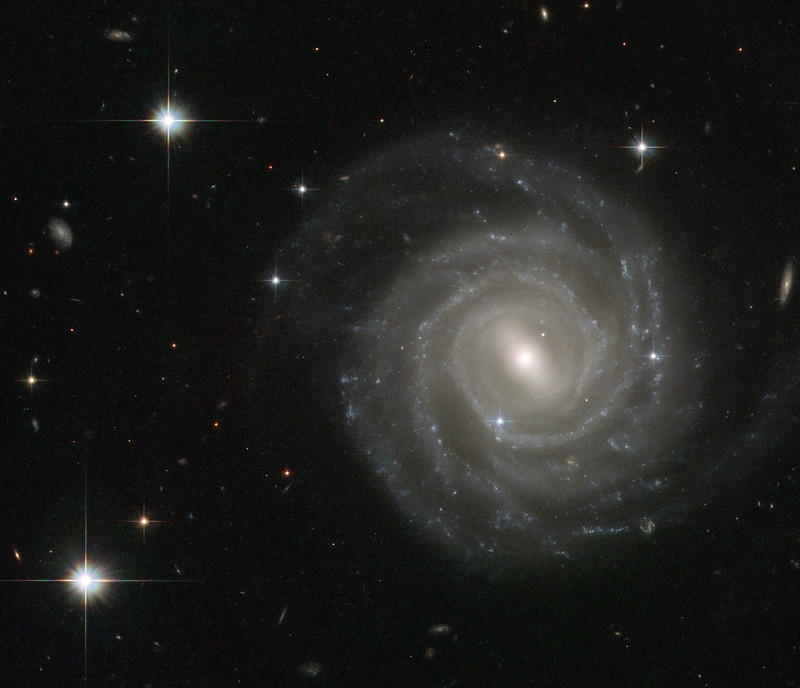
\includegraphics[width=0.8\linewidth]{img/intro/wp/ugc12158.jpg}
%   \caption{UGC 12158 --- галактика с выраженными спиральными рукавами и баром
%     \plholdev{а не барлинза ли тут, кстати}.
%     Пишут что она чем-то похожа на Млечный Путь, а снимок был снят чтобы запечатлеть
%     сверхновую SN 2004e.
%   Credit: ESA/Hubble \& NASA}%
%   \label{fig:frontpic}
% \end{figure}
%
% бессовестно скатано (не без неточностей) из обзора Атанасуллы в Secular evolution in disk galaxies
Как было показано в классических работах \citet{combes1981a} и \citet{raha1991}, вскоре после
образования бара в модели, он <<выгибается>> из плоскости диска и на непродолжительное время теряет симметрию относительно неё. В
результате, галактика при взгляде с ребра показывает ящикообразную или арахисообразную форму, значительное
более утолщённую, чем бар на начальных стадиях формирования. Подобные особенности наблюдались у реальных галактик задолго до их обнаружения в
расчётах и, поскольку они  выступали за плоскость диска, то были названы B/PS (boxy/peanut-shaped) балджами. Например, в статье
\citet{burbidge1959} форма центральной области галактики NGC~128 описана как необычная с наибольшей толщиной не в
центре диска, а в двух симметричных точках по обе стороны от центра\note{``...coming out of the nucleus itself like
a cross''!}, а в \citet{lutticke2000} из $\sim\!1350$ галактик, видимых с ребра, у $45\%$ были найдены B/PS балджи.
На основе многочисленных кинематических исследований была установлена прочная связь между B/PS балджами и внутренней утолщённой в вертикальном направлении частью баров
\citep{kuijken1995,bureau1999,chung2004,bureau2006}. 

С точки зрения наблюдений,
наибольшую сложность представляет задача обнаружить бар в видимой с ребра галактике. В частности, в приведённых выше статьях
было показано, что наличие бара приводит к характерной форме распределения лучевой скорости с двумя высокими пиками и образованию  <<восьмёрки>> на диаграмме $R - v_{\text{loc}}$. 
Подобная корреляция проявляется и при изучении фотометрических характеристик. \citet{lutticke2000a} изучали выборку 60 галактик с B/PS балджами. По форме
профилей яркости в разрезе вдоль большой оси и параллельно ей для 95\% рассмотренных галактик они  подтвердили наличие у галактик бара. 
К тому же, многие B/PS балджи вращаются цилиндрически, что в целом подтверждает их общую природу с баром. 
 
При взгляде на диск галактики <<плашмя>> установить наличие или отсутствие в ней бара гораздо проще, например визуально или по увеличению эллиптичности изофот. Однако, чтобы обнаружить в такой галактике B/PS балдж,  необходима дополнительная информация, например, кинематические данные или металличность звёздного населения. В первом случае в качестве критерия чаще всего используется профиль параметра
$h4$~"---  четвёртого члена в разложении в ряд Гаусса-Эрмита (\cite{vandermarel1993}) распределения лучевой
скорости вдоль большой оси бара. 
О существовании вертикальной арахисообразной структуры говорит наличие на
нём двух симметричных минимумов, обнаруженное в $N$-body моделях \citep{debattista2005,iannuzzi2015}) и наблюдениях \citep{mendez-abreu2008}.

% не менее бессовестно перевел кусок Laurikainen & Salo в книжке Galactic bulges
Однако, не менее интересно понять, к каким отличиям в морфологии бара <<плашмя>> приводит наличие B/PS балджа. 
Инструментом для подобного исследования может выступать анализ изофот, основная идея которого заключается в поиске
их отклонений  от эллипсов~"--- из $N$-body моделей вытекает, что для бара с B/PS балджем,
наблюдаемого на промежуточных углах наклона, изофоты имеют ящикообразную форму\note{не знаю на кого тут
сослаться --- например, Дебатиста 2016, 2017}. Подобным образом с помощью NIR данных из обзора 2MASS  \citet{beaton2007} обнаружили B/PS структуру в галактике M~31 ($i = 77.5^\circ$). В \citet{erwin2013} были изучены 78 галактик с разными углами наклона с целью подобрать оптимальные параметры для
одновременного обнаружения бара и B/PS балджа. При этом, авторы после экстраполяции по выборке
подходящих галактик, пришли к выводу, что 2/3 баров должны проявляться с ребра как B/PS балджи, что в
целом согласуется с выводами \citet{lutticke2000a}, но не очень надёжно в силу небольшого размера выборки.

Для галактик, наблюдаемых под небольшими углами наклона, возможна и отличная от ящикообразной морфология бара.
Довольно часто наблюдаются линзовидные структуры, погруженные в бар в его центральной части. Подобная особенность
была впервые широко освещена в работе \citet{laurikainen2011} и была названа авторами \emph{барлинзой}.
Авторы статьи провели детальную классификацию $\sim\!200$ дисковых галактик ранних типов по данным наблюдений в
инфракрасном диапазоне, добавив условное обозначение для барлинз (bl) в ранее описанные в литературе типы
\citep{devaucouleurs1959,buta2010}). От центральных линз (nuclear lens) и обычных линз они отличаются
размерами, который составляет около половины длины бара, а от классических балджей~"--- профилем плотности и кинематическими
характеристиками. 

Таким образом, бары по их морфологии <<плашмя>> можно разделить на, как минимум, две выделяющиеся группы~"--- бары с
барлинзами и арахисообразные бары. Однако, статистические исследования числа баров разных типов представлены только в
нескольких работах, и пока нет общепризнанного взгляда на этот вопрос. Например, \citet{li2017a} нашли, что при  небольших углах наклона ($0^\circ$ -- $40^\circ$) только $3\%$ процента баров от общего числа изученных объектов имеют арахисообразную форму и $27\%$ демонстрируют морфологию барлинзы. А при больших углах наклона ($40^\circ$
-- $70^\circ$) эти доли составили $13\%$ и $12\%$,  соответственно. При этом доля галактик с баром в обоих
диапазонах отличается незначительно~"--- $74\%$ и $68\%$, так же как и доля галактик, бары в которых имеют
эллиптические изофоты (unbuckled в терминологии авторов). 

Природа барлинз и корреляция между числом баров разных типов на разных наклонениях не могли не вызывать интереса
исследователей в этой области. В статье \citet{athanassoula2013a} приводятся результаты $N$-body моделирования галактик с учетом газа и физических процессов 
в нём (звездообразование, высвечивание и т.п). В модельных галактиках на поздних стадиях эволюции  получилась вполне похожая на барлинзу структура (например, ~Fig.~4 оттуда). В работе  \citet{athanassoula2015} на основе сопоставимих размеров барлинз и B/PS балджей при фотометрической 
декомпозиции $N$-body моделей с учетом газодинамики делается вывод, что это проявления одной и той же структуры, 
видимой под разными углами наклона. В \cite{salo2017} авторы приходят к похожим выводам, анализируя, 
однако, результаты бесстолкновительных расчетов с классическим балджем, заданным в качестве начального условия, а не 
образующимся в результате звездообразования из  натекающего на центр галактики газа. 

Связь наблюдаемой морфологии бара с параметрами подстилающей галактики часто становится предметом исследований, в которых 
анализуются результаты $N$-body расчетов. Так, например \citet{athanassoula2002}  рассмотрели три модели: с массивным гало 
($M_h/M_d = 1.5$), с массивным диском ($M_h/M_d = 0.75$) и с массивным диском и массивным классическим балджем 
($M_h/M_d = 0.75$, $M_b/M_d = 0.6$). При этом, в первом случае образовывался мощный  бар, во втором случае наблюдалось скорее овалообразное искажение изофот, а в третьем~"--- что-то среднее между первым и вторым случаями. В уже упомянутой ранее 
статье \cite{salo2017} авторы отмечают, что кривая вращения с большим градиентом скорости в центральной области, связанная с наличием компактого классического 
балджа или концентрированного темного гало приводит к образованию бара с барлинзой, а более пологая кривая вращения --- при отсутствии балджа~"--- к арахисообразному бару. Важно отметить, что в последнем случае X-образные особенности проявляются даже при нулевом угле наклона (в положении <<плашмя>>).  
\citet{smirnov2018} подтвердили этот вывод и отметили, что варьирование других параметров модели, таких как 
параметр Тумре ($Q$) или начальная толщина диска ($Z_d$) могут приводить к возникновению барлинз в 
бесстолкновительных моделях даже при отсутствии балджа. Однако, приведенные параметры довольно сложно получить из наблюдательных 
данных, в отличие от массы эффективного радиуса балджа, которые определяются из  аккуратной фотометрической декомпозиции 
изображения галактики и анализа звездного населения. Например \citet{laurikainen2014}) для изученной ими выборки галактик нашли, что относительная масса балджа составила
$0.1$, вместо $0.35$, получающейся при неучете в фотометрической декомпозиции  барлинзы. Важно отметить, что и в наблюдениях
\citep{laurikainen2017}, и в моделях \citep{salo2017} возникает промежуточная ситуация~"--- на изображениях с
барлинзами после применения нерезкого маскирования обнаруживаются X-образные детали (Fig~A.4, IC 1067 в первой
статье), причём даже в депроецированных изображениях. Этот факт явно свидетельствуют о динамической природе
морфологических различий. 

Анализ вертикальной структуры $N$-body моделей многокомпонентных галактик показывает связь параметров родительской
галактики с геометрическими параметрами B/PS структур \citep{smirnov2018}, а не только с морфологией бара
<<плашмя>>. Подобная взаимосвязь основана на разнице в орбитальном составе B/PS балджей, образовавшихся в разных
потенциалах \citep{parul2020}. Вопрос об орбитах, поддерживающих трёхмерный бар, достаточно подробно освещён в
литературе (например в обзоре \cite{athanassoula2016}), однако, поскольку барлинзы были обнаружены относительно
недавно, их природа и орбитальный состав ещё во многом остаются неизвестными. 

Цель данной работы~"--- детальное изучение разницы в орбитальном составе различающихся по морфологии баров, которые образуются в самосогласованных $N$-body моделях дисковых галактик. При этом интересовать меня будут именно различия
возникающие при наблюдении плашмя, а вертикальная структура баров не является основным вопросом работы. 
\begin{enumerate}
  \item В главе~\ref{chap:model} описаны параметры $N$-body моделей, приводящие к образованию бара с барлинзой и
    арахисообразного бара и используемая методика проведения $N$-body моделирования,
  \item Глава~\ref{chap:method} посвящена описанию основного метода, используемого в работе~"--- анализа
    доминирующих частот,
  \item Большая часть главы~\ref{chap:split} состоит в описании процедуры выделения орбитальных семейств~"---
    близких по морфологии групп орбит, и в сравнении населённости разных семейств для разных моделей, 
  \item И, наконец, в главе~\ref{chap:orb} приведены основные орбиты для каждого из разобранных семейств.
  \item И, наконец, в главе~\ref{} суммируются полученные результаты делаются основные выводы.
\end{enumerate}

\end{document}
% vim:wrapmargin=3


\chapter{Модели}
\label{chap:model}
\documentclass{trlnotes}
\usepackage{trmath}
\addcompatiblelayout{thesis}
\setlayout{thesis}
\usepackage{trthm}
\usepackage{trsym} 
\usepackage{trphys}
\usepackage{silence}
% \usepackage{tikz}
\WarningFilter{latex}{Reference}
\usepackage[
backend=biber,
sorting=none,
natbib=true,
style=authoryear-comp,
language=russian
]{biblatex}
\addbibresource{../../thesisrefs.bib}
\graphicspath{{../../}}
\begin{document}

Одной из главных задач в численных расчётах является выбор начальных условий. Для того, чтобы изучать природу барлинз и B/PS балджей, необходимо определить, при каких значениях параметров модели они возникают. Для этого необходимо обратиться к результатам наблюдений реальных галактик.

Как уже было описано в предыдущей главе, одним из самых важных параметров, определяющих морфологию бара в положении <<плашмя>>,
является градиент кривой вращения в центральной области, тесно связанный с профилем плотности вблизи центра галактики. В многокомпонентных моделях галактик определённую роль в создании градиента скорости будут играть все компоненты. Следуя за \citet{salo2017}, я буду исследовать только влияние параметров классического балджа, ограничиваясь обычными в литературе NFW-подобными профилями тёмного гало (\cite{navarro1996}). Поскольку барлинзы скорее характерны для дисковых галактиках ранних типов \citep{laurikainen2011}, бедных газом, а B/PS-структуры, в целом, крайне редко встречаются в Scd галактиках \citep{erwin2017, li2017a}\note{В работе \cite{lutticke2000}, однако, описано исключение из этого правила}, можно ограничится бесстолкновительным $N$-body моделированием и не усложнять расчёты учётом 
диссипативной компоненты и сопутствующими ей физическими процессами (как, например, в \cite{athanassoula2015}). 

В работе \citet{salo2017} параметры классического балджа подбирались на основе предыдущих работ этих же авторов по 
фотометрической декомпозиции изображений галактик из инфракрасного (3.6\thinspace μm) обзора S${}^4$G (Spitzer Survey of 
Stellar Structure in Galaxies). \citet{salo2015} в своих моделях брали относительную массу балджа (по отношению к диску), равной  
$M_b/M_d = 0.08$ и $0.01$. При этом эффективный радиус балджа в обоих случаях составлял $0.07$ экспоненциального 
масштаба диска. Такие значения массы балджа могут отличаться примерно в три раза от более ранних оценок, 
встречающихся в литературе, в силу особенностей фотометрической декомпозиции, таких как учёт барлинз и B/PS 
балджей \citep{laurikainen2016a}, но при этом, например, в работе \citet{erwin2015} получены сходные результаты для 
композитных балджей, состоящих из классического балджа и псевдобалджа. Таким образом, оценка $M_b/M_d = 0.01 \div 
0.1$ согласуется с современными наблюдательными данными.

В данной работы были рассмотрены четыре модели с разными параметрами классического балджа при неизменности параметров остальных компонент.  Методом проб и ошибок было обнаружено, что подобранные параметры обеспечивают плавный переход между разной морфологией бара, что очень важно для изучения возникающих различий. 

За основу были взяты результаты $N$-body расчётов из работы 
\citet{smirnov2018}. % и к ним добавлены новые расчёты.
Модели включали в себя экспоненциальный диск:
\begin{equation}
  \label{eq:rho_disk} \rho_d(R,z) = \frac{M_d}{4\pi R_d^2 z_d} \cdot \exp(-R/R_d) \cdot \sech^2(z/z_d)\,,
\end{equation}
где $R$~"--- цилиндрический радиус, $M_d$~"--- полная масса диска, $R_d$, $z_d$~"--- радиальный и вертикальный 
масштабы диска, соответственно. Начальный профиль радиальной дисперсии скорости тоже экспоненциальный:
\begin{equation}
  \label{eq:sigma_disk} σ_R = σ_0 \cdot \exp (-R/R_σ), \quad R_σ = 2 R_d, 
\end{equation}
$σ_0$ определена так, чтобы параметр Тумре \citep{toomre1964} на 
радиусе $R_σ$ был равен некоторому заданному значению.  Точные 
значения параметров для всех моделей приведены в 
таблице~\ref{tab:modelpars}.
В дальнейшем изложении для удобства мы будем пользоваться системой 
единиц, в которой $R_d = 1$, $M_d = 1$, $G = 1$. Приняв $R_d = 
3.5\,\text{кпк}$, $M_d = 5\cdot 10^{10}\,\solmass$, получим единицу 
времени, равной $\sqrt{\frac{R_d^3}{GM_d}}\approx 13.81\, \text{млн. лет}$. Единица частоты в этом случае~"--- 
$163.95\,\text{км}/\text{с}/\text{кпк}$.  

Тёмное гало в моделях задаётся усечённым профилем плотности, похожим на профиль NFW (\cite{navarro1996}):
\begin{equation}
  \rho_h(r) = \frac{C_h}{(r/r_s)^{\gamma_0}\left((r/r_s)^\eta+1\right)^{(\gamma_\infty-\gamma_0)/\eta}} \,, \label{eq:NFW}
\end{equation}
где $r_s$~"--- радиальный масштаб гало, принятый равным 6, $η$ 
описывает форму профиля во внешней области, $γ_0$ и 
$γ_{\infty}$~"--- внутренний и внешний наклон профиля, 
соответственно, а $C_h$ задаёт полную массу гало $M_h$. Были 
приняты следующие значения параметров профиля гало:
$η = 4/9$, $γ_0 = 7/9$, $γ_∞ = 31/9$~"---  более пологий в центральной области и более крутой на периферии, чем 
оригинальный профиль Наварро-Фрэнка-Уайта. $C_h$ выбрано так, чтобы $M_h(r < 4R_d) = 1.5$. 

\begin{table}[htpb]
  \centering
  \caption{Параметры рассматриваемых $N$-body моделей. Приведены в порядке увеличения концентрации балджа.}
  \label{tab:modelpars}
  \vskip 2ex
  \begin{tabular}{cr|ccccccc}
  \toprule
     & Модель & $z_d$ & $Q$ & $M_h$ & $M_b$ & $r_b$ & $\del v_{cb}/\del r \, (r_b/2)$ & \\
  \midrule
     &X   & $0.05$ & $1.2$ & $1.5$ & $0$ &  &  &\\
     &Xbl & $0.05$ & $1.2$ & $1.5$ & $0.2$ & $0.2$ & $0.79$ &\\
     &BLx & $0.05$ & $1.2$ & $1.5$ & $0.1$ & $0.1$ & $1.57$\\
     &BL  & $0.05$ & $1.2$ & $1.5$ & $0.1$ & $0.05$ & $4.44$ &\\
  \bottomrule
  \end{tabular}
\end{table}

В три из четырёх моделей в качестве дополнительного потенциала был добавлен потенциал классического балджа, 
задаваемый профилем\note{Этот профиль является хорошим приближением закона де Вокулёра.} \citep{hernquist1990}: 
\begin{equation}
  \rho_b(r) = \frac{M_b\, r_b}{2\pi\,r\,(r_b + r)^3} \,,
\end{equation}
где $M_b$~"---полная масса балджа, а $r_b$ задаёт его характерный размер.  Принятые значения параметров балджей 
приведены в таблице~\ref{tab:modelpars}.
Зная профиль плотности, можно получить потенциал:
\[
  Φ(r) = -\frac{M_b}{r+r_b},
\]
а затем модельную кривую вращения:
\[
  v_{cb}(r) = \sqrt{r \, \fder{Φ}{r}} = \sqrt{\frac{M_b\, r}{(r + r_b)^2}} \,. 
\]
Из кривой вращения оценим её градиент в центральных областях, например, на расстоянии $r_b/2$.
\[
\left. \fder{v_{cb}}{r} \right|_{r=r_b/2} = 
\left. \sqrt{\frac{M}{r}}\, \frac{r_b-r}{2\, (r_b+r)^2} \right|_{r=r_b/2} = 
\sqrt{\frac{M}{r_b^3}}\, \frac{\sqrt{2}}{9}
\]
Из последнего равенства видно, что именно средняя концентрация балджа определяет наклон кривой вращения, и, как 
следствие, морфологию бара.

В $N$-body расчётах особое внимание следует уделять влиянию численных эффектов. В частности, при малом количестве 
частиц сильно уменьшается время релаксации, что ведёт к динамической эволюции модели, которая не соответствует 
процессам в реальных галактиках. В моделях, используемых в данной работе, диск состоял из $N_d = 4\cdot 10^5$ 
частиц, а гало из $N_h=4.5\cdot 10^5$; обоснование этого выбора можно найти в \citet{smirnov2018}.  Равновесная 
модель, соответствующая описанным начальным условиям, была подготовлена с помощью скрипта \texttt{mkgalaxy} 
\citep{mcmillan2007a}. Длина сглаживания потенциала для диска и гало принята равной $ε_d = 3.7\cdot 10^{-3}$ 
($\approx 13 \text{пк}$) и $ε_h = 12.9\cdot 10^{-3}$ ($\approx 45 \text{пк}$) соответственно.  Эти значения согласуются с результатами статьи \citet{salo2017}. В ней авторы анализировали  изменения морфологии бара в зависимости от длины сглаживания и получили, что больших $ε_d$ барлинза замывается. Для корректного моделирования барлинзы необходимо $ε_d<0.05$ в соответствующей модели с балджем, так как $ε_d < 0.05$.

Эволюция модели изучалась с помощью интегратора \texttt{gyrfalcON} \cite{dehnen2002}, использующего комбинацию
tree-code метода и мультипольного разложения, с асимптотической сложностью алгоритма $\mathcal O(N)$. Этот код 
является частью свободного пакета \texttt{NEMO} \citep{teuben1995a}, предоставляющего набор утилит для $N$-body 
моделирования. В каждой из 4 моделей в первоначальном осесимметричном диске довольно быстро формируется бар. К моменту $t=400$ бар уже вырос в 
вертикальном направлении и медленно меняет свою амплитуду и скорость узора% (\ref{fig:4models}).
Для изучения его орбитальной структуры в следующих главах мы будем использовать методы спектральной динамики, впервые описанные в работе 
\citet{binney1982}. Эти методы основаны на поиске доминирующих частот в Фурье-спектрах временных рядов координат частиц. При этом необходимо 
достаточно высокое временное разрешение. Оно было достигнуто пересчётом моделей на промежутке времени с $t=400$ до $t=500$ с очень маленьким 
шагом по времени, а также за счёт малости изменения посчитанных частот на этом промежутке. На основе оценок, приведённых в \cite{parul2020}, на 
рассматриваемых временах бар эволюционирует медленно, и характерная величина сдвига частот сравнима с ошибками определения частот на сетке, что 
и позволяет проводить относительно надёжный анализ.

\end{document}
% vim:wrapmargin=3 formatoptions=aw2tq


\chapter{Метод анализа частот}
\label{chap:method}
\documentclass{trlnotes}
\usepackage{trmath}
\addcompatiblelayout{thesis}
\setlayout{thesis}
\usepackage{trthm}
\usepackage{trsym} 
\usepackage{trphys}
\usepackage{silence}
% \usepackage{tikz}
\usepackage[
backend=biber,
sorting=none,
natbib=true,
style=authoryear-comp,
language=russian
]{biblatex}
\addbibresource{../../thesisrefs.bib}
\graphicspath{{../../}}
\begin{document}

Существование структур в моделях, сохраняющихся на масштабах времени $10^9$ лет, возможно лишь при наличии стабильных околопериодических орбит. Эти орбиты и определяют  общую морфологию структур. Такие орбиты должны лежать недалеко друг от друга в фазовом пространстве. Мы будем называть их орбитальными семействами. 

Более точное определение семейства зависит от рассматриваемого представления фазового пространства. В классической литературе, посвящённой анализу орбит в модельных
потенциалах в двумерном случае \citep{contopoulos1980a,2008gady.book.....B}, в качестве фазового пространства используют чаще всего сечения Пуанкаре. Однако такой подход плохо подходит для изучения $N$-body моделей~"--- орбиты частиц трёхмерные, и их энергии могут принимать значения в широком диапазоне. Оба этих фактора приводят к <<размытию>> сечений Пуанкаре и усложняют задачу
классификации орбит \citep{valluri2016}. Поэтому в настоящей работе используется другой метод представления фазового
пространства~"--- двумерные распределения отношений доминирующих частот (frequency map). 

Попробуем разобраться в физическом смысле такого распределения. Перейдём к координатам действие-угол: $(J_i,
\theta_i)$. Тогда из определения интеграла движения и уравнений Гамильтона получим 
\[
  0 = \dot J_i = -\pder{H}{θ_i} \so \dot θ_i = \pder{H}{J_i} =
  Ω_i(\v J) = \text{const} \so θ_i(t) = θ_i^0 + Ω_i \,t
\]
Ограничиваясь замкнутыми орбитами (все остальные быстро покидают систему и не могут образовывать долгоживущую
структуру), можно записать разложение декартовых координат в ряд Фурье
\[
  x_i (t, \v J) = \sum_{\v n\in \Z^m} X_{i,n} (\v J)\, e^{i\,\mathbf{n}\cdot \v θ^0}\, e^{i\,\v n\cdot \v Ω\,t}\,,
\]
определяемый набором \emph{фундаментальных} частот: $\{Ω_i(\v J)\}_i$. Орбита называется \emph{резонансной}, если
её фундаментальные частоты соизмеримы: $\exists\, n \neq 0\that \v n \cdot \v Ω = 0$. В координатах действие-угол
траектории частиц <<наматываются>> на торы, задаваемые интегралами движения частиц (например, полная энергия, угловой момент), при этом нерезонансные орбиты заметают весь тор, а квазипериодические~"--- ограниченную область на нем. Это
фактически означает, что для них есть свой интеграл, который понижает размерность резонансного семейства в фазовом
пространстве. Таким образом, резонансные орбиты структурируют фазовое пространство, и представляется
естественным классифицировать орбиты, опираясь на эту структуру в фазовом пространстве как <<скелет>> структуры в обычном пространстве.

Подобный подход часто встречается в литературе. Можно сослаться на классическую работу \citet{binney1982} и более
современные работы  \citep{athanassoula2002,portail2015,valluri2016}. Подробно этот подход описан в обзоре
\citet{athanassoula2013}. Общая идея частотного анализа состоит в поиске пиков на спектрах координат и цилиндрического
радиуса $R = \sqrt{x^2 + y^2}$. Положение пиков используется для  вычисления исследуемых частот.  При этом, чаще всего
изучаются орбиты либо в аналитических потенциалах, либо в потенциалах из $N$-body моделирования, но <<замороженных>> на
какой-то фиксированный момент времени. В обоих случаях потенциалу искусственно придаётся вращение с угловой скоростью
бара. Необходимость этого обусловлена требованием независимости интегралов движения от времени, что может не
выполняться в самосогласованных $N$-body расчётах на больших промежутках времени.  Однако, в
работе \citet{ceverino2007}
был применён другой, более трудоёмкий, но более <<честный>> подход~"--- авторы изучали орбиты непосредственно в
<<живом>> $N$-body потенциале, но на таком интервале времени, где потенциал галактики и скорость вращения бара
изменяются незначительно. При этом пики на спектрах естественно размываются, но полученные авторами результаты качественно совпадали с результатами стандартного подхода \citep{athanassoula2002a}.  Мы будем использовать сходную методику, во многом следуя работе \citet{gajda2016}. Результаты этой работы, по-видимому, ближе всего соответствуют структуре реальных галактик.

Орбитальное движение частиц в модели рассматривается в системе отсчёта, вращающейся вместо с баром. Ось $x$ направлена
вдоль большой оси бара, $z$ перпендикулярна плоскости диска, а $y$ дополняет их до правой тройки.  Для каждой из $4\cdot
10^6$ частиц диска строятся временные ряды $\{x_k(t), y_k(t), z_k(t), R_k(t)\}$ от $t_1=400$ (5.3 млрд. лет) до
$t_2=500$ (6.6 млрд. лет) с шагом $Δt = 0.125$ единиц, после чего, с помощью кода, написанного аспирантом СПбГУ
Смирновым~А.А., вычисляются частоты, соответствующие пикам на периодограмме с наибольшей амплитудой. Вычитая из
изначального ряда сигнал, модулированный основной частотой, и вычисляя периодограмму разности, можно определить второй по
величине пик и так далее. Всего выделялось три пика, но анализ орбитальных семейств в основном производился по первым
пикам, с привлечением вторых.

\begin{figure}[htpb]
  \centering
  \includepgfgraphics[height=7cm]{img/method/orbit-3793601-xy.pgf}
  \includepgfgraphics[height=7cm]{img/method/orbit-3793601-timeseries.pgf}
  \includepgfgraphics[height=7cm]{img/method/orbit-3793601-spectra.pgf}
  \caption{Пример спектра для одной из орбит вблизи центра модели. Сверху: временные ряды $x(t)$, $y(t)$, $R(t)$ на промежутке
  $[400; 420]$, снизу: соответствующие им периодограммы. Промежуток времени выбран так, чтобы отдельные кривые были
  различимы на графике, вычисление частот идёт на всем доступном промежутке $[0;100]$.
  }%
  \label{fig:spectrasample}
\end{figure}

Из-за дискретности временного ряда, максимальное возможное значение частоты ограничено частотой Найквиста: 
\[
  ν_c = \frac{1}{2 Δt} = 4, \quad ω_c = 2\pi ν_c \approx 4120\,\text{км}/\text{с}/\text{кпк}\,,
\]
Однако, даже для орбит вблизи центра модели, вычисленные значения частот много меньше частоты Найквиста
и алиасинга не происходит (рис.~\ref{fig:spectrasample}).

Ограниченная длина временного ряда приводит к ограниченному разрешению по частотам: 
\[
  Δν = \frac{1}{t_2 - t_1} = 0.01, \quad Δω = 2\pi Δν \approx 10\,\text{км}/\text{с}/\text{кпк}.
\]
При этом, вторая величина определяет точность определения пиков на спектре, и для аккуратного выделения резонансных
орбит её не достаточно.  Используемый алгоритм решает эту проблему следующим образом. Сначала находятся положения пиков
на изначальной сетке частот, а потом пересчитывается преобразование Фурье в окрестности пика с шагом $Δ_1ν = 0.001$, т.е. в 10 раз меньшим, чем изначальный.
Являясь разновидностью схемы дополнения временного ряда нулями, такой способ не позволяет различить сливающиеся на
грубой сетке пики, однако десятикратно увеличивает точность определения положения одиночного пика. Более полно детали
алгоритма и оценка дрейфа частот описаны в \citet{parul2020}. Для моделей, анализируемых в моей работе, на заданном
временном интервале скорость дрейфа меньше, чем $0.01$~"--- разрешение изначальной сетки.

В следующей главе будет подробно описан процесс выделения различных орбитальных семейств с помощью отношений полученных
частот ($ω_x, ω_y, ω_z, ω_R$) для всех моделей. Перед этим важно отметить, что используемый метод не позволяет
\emph{точно} разделить резонансные, квазипериодические и близкие к ним, но хаотические орбиты просто в силу
ограниченного разрешения по частоте. Поэтому, в одно семейство мы будем выделять сходные по морфологии орбиты с
довольно близкими отношениями частот, используя при этом всю доступную информацию, например амплитуды соответствующих
пиков периодограммы. Подобная проблема не так выражена в модельных или замороженных потенциалах, не подверженных
долговременной эволюции, однако исследования таких потенциалов носят всё же академический характер и не дают полного
понимания орбитальной структуры <<живой>> модели.

\end{document}
% vim:wrapmargin=3


\chapter{Выделение семейств}
\label{chap:split}
\documentclass[tikz]{trlnotes}
\usepackage{trmath}
\addcompatiblelayout{thesis}
\setlayout{thesis}
\usepackage{trthm}
\usepackage{trsym} 
\usepackage{trphys}
\usepackage{silence}
% \usepackage{tikz}
\usepackage[
backend=biber,
sorting=none,
natbib=true,
style=authoryear-comp,
language=russian
]{biblatex}
\addbibresource{../../thesisrefs.bib}
\WarningFilter{latex}{Reference}
\graphicspath{{../../}}
\begin{document}
В работах, посвящённых классификации орбит на основе доминирующих частот, часто используются набор из угловой
частоты $Ω$, эпициклической частоты $ϰ$ и вертикальной частоты $ν$
\citep{athanassoula2002a,ceverino2007,voglis2007}. Однако для изучения структуры бара во вращающейся системе
отсчёта гораздо удобнее рассматривать <<декартовы>> ($ω_x, ω_y, ω_z, ω_R$) частоты, введённые в предыдущей главе, и не использовать угловую частоту $Ω$, определение которой не очень точно и требует учёта дополнительной информации кроме спектров
\citep{athanassoula2002,gajda2016}. К тому же, \citet{valluri2016} показали, что, по крайней мере, в <<замороженных>> потенциалах отношения декартовых частот
гораздо лучше разделяют орбитальные семейства. 
Однако, все-таки полезно сопоставить одни частоты с другими для лучшего понимания физики происходящего. Соотношения между ними такие: 
\[
  ω_x \approx Ω - Ω_p, \quad ω_z = ν, \quad ω_R = ϰ,
\]
где $Ω_p$~"--- скорость вращения бара. Из-за постепенного замедления вращения бара и возможного вклада вторых частот первое равенство оказывается приближённым, а остальные два верны просто по определению.

Перед тем как начать классифицировать семейства, необходимо сузить рассматриваемое множество частиц до наиболее
интересных. Предварительная обработка модели включала следующие этапы.
\begin{enumerate}
  \item Отделение диска от гало. 
  \item Перенос начала отсчёта координат в центр масс диска.
  \item Переход в систему отсчёта, вращающуюся вместе с баром.
  \item Выбор интересующей нас области диска, где расположен бар.
\end{enumerate}
Первые три этапа были выполнены с помощью пакета \texttt{NEMO}, после чего был произведено вычисление доминирующих частот, как об этом было сказано в главе \ref{chap:method}. Опишем теперь более 
подробно четвёртый шаг.
\paragraph{Отделение диска и выбор области, связанной с баром}

В силу выбора координатных осей, связанных с баром, в модели возникает характерный радиус, на котором угловая скорость вращения системы отсчёта практически совпадает с угловой скоростью вращения частиц в диске.
В окрестности этого радиуса абсолютные значения доминирующих
орбитальных частот $\omega_x$ и $\omega_y$ окажутся малыми, порядка $\frac{2\pi}{t_2 - t_1}$, поскольку частица не успевает совершить полный оборот вокруг центра на отрезке времени, для которого строится временной ряд и вычисляется преобразование Фурье. Естественно отождествить этот радиус с радиусом
коротации в модели (CR). Обозначим его через $R_c$ и выделим три группы частиц по их расположению относительно коротации
(Рис.~\ref{fig:disksplit}, внизу)\note{В качестве вертикальной оси
выбран $|ω_x|$, поскольку именно эта величина вычисляется
алгоритмом. В дальнейшем изложении модуль опускается, поскольку
внутри коротации $ω_x > 0$.}.
\begin{enumerate}
  \item $|ω_x| < |ω_{x, \min}| \:\lor\: |ω_y| < |ω_{x, \min}|$.
Частицы из этой группы образуют кольцо с утолщениями в
симметричных точках на оси $y$ вблизи радиуса коротации, закрашенное в верхней части рис.~\ref{fig:disksplit}
оранжевым цветом.
Очень похожая структура была обнаружена в работе \citet{ceverino2007}, но по критерию $Ω \approx Ω_p$, который, на мой взгляд, сложнее. В упомянутой работе подробно описывается <<захват>> частиц на коротации, который
наблюдается и в наших моделях. С точки зрения аналитических моделей потенциалов, он связан с устойчивостью
точек Лагранжа $L_4$ и $L_5$ \citep[Fig.~3.14]{2008gady.book.....B}; утолщения на кольце наблюдаются в окрестности этих точек.
В качестве радиуса коротации принималась середина кольца.  
\item Частицы с $|ω_x| > |ω_{x, \min}| \land |ω_y| > |ω_{y, \min}|$, находящие дальше коротации, связаны с диском
(рис.~\ref{fig:disksplit}, зелёный цвет). Поскольку нас интересует только орбитальный состав бара, они были сразу исключены из рассмотрения. 
\item Частицы с $|ω_x| > |ω_{x, \min}| \land |ω_y| > |ω_{y, \min}|$,
  находящие внутри коротации, представляют наибольший интерес в данном
  исследовании. В классической работе \citet{contopoulos1980} было
  показано, что основные орбиты, составляющие
бар не могут заходить за радиус коротации, поэтому, ограничив рассмотрение только этой областью, мы ничего не
упустим.
\end{enumerate}

\begin{figure}[htpb]
  \centering
  \includepgfgraphics[width=0.77\linewidth]{img/families/bulge1.5c/discsplit-proj.pgf}\par
  \includepgfgraphics[width=0.77\linewidth]{img/families/bulge1.5c/discsplit-cr.pgf}
  \caption{Разбиение частиц на области на примере модели BL.
    Верхний рисунок иллюстрирует разбиение в проекции ($x$, $y$).
    На нижнем --- показан профиль величины $|ω_x| \approx |Ω - Ω_p|$ (в зависимости от среднего радиуса орбиты) и схематично продемонстрирован выбор радиуса коротации. Все рисунки сделаны на момент времени $t=450$.
Детали процедуры разбиения описаны в тексте.}%
  \label{fig:disksplit}
\end{figure}

Однако, как можно заметить на рис.~\ref{fig:disksplit}, даже во внутренней части всё ещё остаются частицы, мало
связанные с баром. Особенно хорошо это заметно в проекции $(x, z)$, где, помимо утолщённой части бара, остаются
частицы лежащие вблизи $z=0$. Нельзя исключать возможность, что такие частицы все же принадлежат бару (например, т.н.
ansae~"--- <<ручки>>, соединяющие бар с кольцом), поскольку размеры B/PS структуры меньше длины самого бара. Однако, как
уже было описано во Введении, барлинзы и B/PS балджи имеют сходные размеры, поэтому возможная потеря концов бара
вряд ли изменит его морфологию, наблюдаемую <<плашмя>>. 

\begin{figure}[htpb]
  \centering
  \begin{tikzpicture}[
    im/.style = {inner sep=0pt, text width=0.8\textwidth},
    node distance = 10pt
    ]
    \node[im] (FxFz) at (0,0) [anchor=south west] {\includepgfgraphics[width=\textwidth]{img/families/bulge1.5c/cl_fxfz.pgf}}; 
    \node[im] [below=of FxFz] {\includepgfgraphics[width=\textwidth]{img/families/bulge1.5c/m_Ravfzfx.pgf}}; 
    \begin{scope}[x={(FxFz.south east)},y={(FxFz.north west)}]
      \coordinate (origin) at (0.126,0.111);
      \coordinate (x1y2) at (0.87,0.97);
      \draw[very thick,red!30!black] let \p1 = ($ (x1y2) - (origin) $) in 
        (origin)  -- + (0.89*\x1, \y1);
    \end{scope}
  \end{tikzpicture}
  \caption{Двумерные карты частот. Вверху: двумерное распределение
    $ω_x$ -- $ω_z$. Тёмно-красная прямая на рисунке соответствует условию
    $ω_z = 2.25\, ω_x$ (исключается все слева от неё). Внизу: двумерное
    распределение отношения $ω_z/ω_x$ -- средний радиус
  орбиты $\averg{R}$ (исключается область выше $ω_z/ω_x = 2.25$ и правее $\averg{R} = 0.8$).}
  \label{fig:innerrefine}
\end{figure}

Опишем процедуру выбора исследуемой внутренней области диска. На верхней части рис.~\ref{fig:innerrefine} можно
заметить выделяющуюся прямую, соответствующую орбитам с $ω_z = 2\, ω_x$, <<полосу>> правее неё с меньшим отношением
$ω_z /ω_x$ и область вблизи $ω_x = 0$ с большими значениями этого отношения. Нижняя часть рис.~\ref{fig:innerrefine} ясно демонстрирует, что эта область состоит из двух частей~"--- орбиты с небольшими значениями $\averg{R}$ вблизи начала координат и <<хвост>> орбит, уходящих далеко от центра. Именно эти орбиты лежат вблизи $z=0$, как хорошо видно на рис.~\ref{fig:inneredgeon}. В итоге, из изначально выбранной области
внутри коротации дополнительно отбираются орбиты по критериям
\begin{equation}
  ω_z/ω_x < 2.25 \: \lor \: \averg{R} < 0.8.
\end{equation}
В дальнейшем я буду изучать только ту часть области внутри коротации, для
которой выполнен вышеприведённый критерий, поскольку остальная часть
диска не представляет интереса для исследования орбитального состава
внутренних областей бара, наблюдаемого <<плашмя>>. При этом, для всех
четырёх моделей рассматриваемая часть содержит около $50\%$ от 4 млн.
частиц диска. Для неё было принято обозначение ROI. 
\begin{figure}[htpb]
  \centering
  \includepgfgraphics[width=0.48\linewidth]{img/families/bulge1.5c/xy_hex.pgf}
  \includepgfgraphics[width=0.48\linewidth]{img/families/bulge1.5c/other/xy_hex.pgf}
  \\
  \includepgfgraphics[width=0.48\linewidth]{img/families/bulge1.5c/xz_hex.pgf}
  \includepgfgraphics[width=0.48\linewidth]{img/families/bulge1.5c/other/xz_hex.pgf}
  \caption{Проекции частиц внутри коротации на плоскости $(x,y)$ (вверху) и $(x,z)$ (внизу) на момент времени $t=450$. Слева: выбранная для анализа область, справа: оставшаяся часть внутри коротации. Цветовая шкала совпадает на изображениях в одном ряду: для верхнего ряда максимальное значение составляет $5000$, для нижнего~"--- $7500$.%
  }%
  \label{fig:inneredgeon}
\end{figure}

\paragraph{Основные семейства}
\tikzset{
  modelname/.style = {
    fill=lightgray, fill opacity=0.8, text opacity=1,
    font=\Large
}}
Опишем в деталях процедуру выбора орбитальных семейств. 
Поскольку задачей является получение единообразной и максимально полной классификации орбит, объясняющей все рассмотренные варианты морфологии бара, необходимо сначала хотя бы на качественном уровне понять, какие семейства можно выделить во всех моделях по отношению доминирующих частот. На рис.~\ref{fig:modelcomp1dist} приведены проекции области,
выбранной по алгоритму, описанному выше, на плоскость $(x,y)$ для всех 4-х моделей (слева) и одномерные распределения отношений $ω_R/ω_x$, $ω_y/ω_x$. Хорошо заметен пик вблизи
2 для первого из распределений частот и вблизи 1 для второго. Поскольку в выбранной системе отсчёта $ω_x \approx Ω - Ω_p$, можно, следуя работам \citet{gajda2016,portail2015}, отождествить $ω_R \approx 2\, ω_x$ с баром в его классическом
понимании, составленном из орбит\note{Более подробное обсуждение типов орбит изложено в главе~\ref{chap:orbits}},
порождённых так называемым семейством $x_1$ и находящихся в внутреннем резонансе Линдблада (ILR) \citep{athanassoula2003}.
Важно отметить, что использование критерия, завязанного на декартовы частоты, не искажает морфологию получившегося <<классического>> бара. Представленные в дальнейшим изложении
проекции этого семейства очень похожи на изображения ILR в работе \citet[Fig.~10]{ceverino2007}, отождествлённого по условию $Ω - Ω_p \approx ϰ/2$. Слева и справа от пика в $2$ на распределении $ω_R/ω_x$ отчётливо видны ещё как минимум два семейства:
с $ω_R/ω_x > 2$ и $ω_R/ω_x < 2$.  По мере перехода от арахисообразной формы бара к бару с линзой их
относительный вклад увеличивается, а количество частиц, находящихся на
ILR уменьшается. 
% нет, не было показано.
%Наблюдается важное отличие между моделями BL и BLx~"---
%для семейства с $ω_R/ω_x < 2$ возникает довольно широкий пик на распределении $ω_R/ω_x$ вблизи $ω_R/ω_x \approx 1.7$. Как будет показано в дальнейшем, именно семейство, сооотвествующее этому пику, вносит наибольний вклад в округлую форму, присущую барлинзе.

Не менее интересная закономерность наблюдается и на распределениях отношения частот $ω_y/ω_x$. Широкая область справа от пика в единице,
соответствующая т.н. boxy орбитам, становится всё менее протяжённой по значению отношения и менее населённой. На каждом графике в этой области
можно выделить свой небольшой пик, соответствующий резонансным орбитам. В терминологии, принятой в статье \cite{valluri2016}, такие орбиты
называются resonant boxlet орбитами. Для модели с арахисообразным баром маленький пик соответствует $ω=5/3$, для промежуточных морфологий~"--- $3/2$, а для бара с барлинзой~"--- $4/3$.
За счёт уменьшения количества boxy орбит возрастает величина пика с $ω_y/ω_x = 1$. Значительную его часть
составляют орбиты, генетически связанные с семейством $x_1$ и ответвлениями от него в вертикальном направлении, находящиеся в баре.

Обобщая качественные рассуждения, изложенные выше, можно,  сформулировать следующие критерии <<автоматической>> (в
таком же смысле как в \cite{valluri2016}) классификации орбитальных семейств. Эти критерии вместе с условным обозначением для каждого семейства приведены ниже.
Границы семейств были выбраны на основе результатов статьи \citet{portail2015}, поскольку другие методы (например, по погрешности отношения) настолько же нефизичны и не позволяют получить универсальную оценку, не зависящую от радиуса.
\begin{table}[htpb]
    \centering
  \begin{tabular}{r|l}
    \toprule
    {семейство}   & критерий \\
    \midrule
    ILR & $|ω_R/ω_x - 2| < 0.1$ \\
    $x_i$ bar & $|ω_R/ω_x - 2| < 0.1 \land |ω_y/ω_x - 1| < 0.1$ \\
    boxy bar  & $|ω_R/ω_x - 2| < 0.1 \land  ω_y/ω_x > 1.1$ \\
    $\text{bl}_\text{u}$  & $ω_R/ω_x < 1.9$ \\
    $\text{bl}_\text{o}$  & $ω_R/ω_x > 2.1$ \\
    \bottomrule
  \end{tabular}
  \caption{Обозначения и критерии выделения для рассматриваемых орбитальных семейств.}
  \label{tab:orbfamiles}
\end{table}

\begin{figure}[htpb]
\centering
\begin{tikzpicture}[
  snap/.style = {inner sep=0pt, text width = 0.2\textwidth},
  dist/.style = {inner sep=0pt, text width = 0.4\textwidth},
  node distance = 0.1cm,
  ]
  \node[snap] (X)     at (0,0)     {\includepgfgraphics[width=\textwidth]{img/families/nbulge1.5/xy_hex_nl.pgf}};
  \node[snap] (Xbl) [below=of X,  yshift=-1.5cm]{\includepgfgraphics[width=\textwidth]{img/families/bulge1.5m/xy_hex_nl.pgf}};
  \node[snap] (BLx) [below=of Xbl,yshift=-1.5cm]{\includepgfgraphics[width=\textwidth]{img/families/bulge1.5/xy_hex_nl.pgf}};
  \node[snap] (BL)  [below=of BLx,yshift=-1.5cm]{\includepgfgraphics[width=\textwidth]{img/families/bulge1.5c/xy_hex_nl.pgf}};
  \foreach \modelname\alias in {X/nbulge1.5, Xbl/bulge1.5m, BLx/bulge1.5, BL/bulge1.5c}{
    \node[modelname, anchor=north west, xshift=2pt, yshift=-2pt] at (\modelname.north west) {\modelname}; 
    \node[dist] (\modelname fy/fx) [right=of \modelname,yshift=-0.2cm] {\includepgfgraphics[width=\textwidth]{img/families/\alias/p_dNfyfx.pgf}};
    \node[dist] (\modelname fR/fx) [right=of \modelname fy/fx]         {\includepgfgraphics[width=\textwidth]{img/families/\alias/p_dNfRfx.pgf}};
  }
\end{tikzpicture}  
\caption{Морфология бара и одномерные распределения отношений доминирующих частот для всех 4 моделей. В левой колонке:
  $(x,y)$ проекции интересующей области в квадрате $[-3;3]\times[-3;3]$, в центре: распределение отношения $ω_y/ω_x$ с шириной бина $0.01$, справа: распределение отношения $ω_R/ω_x$ с шириной бина $0.01$. По мере перехода от арахисообразного бара (X) к барлинзе (BL) заметно понижение высоты пика, соответствующего бару в классическом
  смысле, и увеличение высоты пиков для не принадлежащих ему семейств. Уменьшается также и количество boxy орбит.}
\label{fig:modelcomp1dist}
\end{figure}

Более наглядно разбиение на семейства видно на двумерных картах отношений
доминирующих частот, показанных на рис.~\ref{fig:fRfxfRfy_bar}.
Сопоставляя выделенные семейства с <<лучами>> на иллюстрации в его правой
части, можно заметить, что орбиты, попавшие в $\text{bl}_{\text{o}}$,
разбиваются на две группы: с $ω_x + ω_y \approx ω_R$ и с $ω_x \approx
ω_y$. Семейство из первой группы было отмечено в работе \citet{gajda2016}
как семейство, не поддерживающее бар. Но при этом авторы включают в него
и не попавшие ни в одну из выделенных ими групп орбиты с $ω_y/ω_x < 1.2$,
для которых амплитуда наибольшего пика на периодограмме $y$ координаты
больше аналогичной величины для $x$. Внимательно изучив форму изофот на
проекциях всех частиц семейств, я не обнаружил реальной разницы между
верхним и нижним лучом. По этой причине в данной работе обе этих группы
объединены в одно семейство  $\text{bl}_\text{o}$. Примеры орбит,
приведённые в следующей главе, подтверждают осмысленность такого решения.

\begin{figure}
\centering
% \begin{minipage}{.23\textwidth}
\begin{tikzpicture}[
  annotation/.style = {
    fill=lightgray, fill opacity=0.8, text opacity=1,
    rounded corners=3pt
  },
  preview/.style = {inner sep=0pt, text width=0.2017\textwidth},
  overview/.style = {inner sep=0pt, text width=0.78\textwidth},
  node distance = 0pt
  ]
  \node[overview, anchor=south west] (BL) at (0,0) %
    {\includepgfgraphics[width=\textwidth]{img/families/bulge1.5c/2dpr_fxfRfyfR.pgf}};
  
  \node[preview]  (Xb)  [left=of BL,xshift=-0.018\textwidth, yshift=0.029\textwidth] %
    {\includepgfgraphics[width=\textwidth]{img/families/bulge1.5m/2dpr_fxfRfyfR_nl.pgf}};
  \node[preview]  (X)   [above=of Xb]  %
    {\includepgfgraphics[width=\textwidth]{img/families/nbulge1.5/2dpr_fxfRfyfR_nl.pgf}};
  \node[preview]  (BLX) [below=of Xb] {\includepgfgraphics[width=\textwidth]{img/families/bulge1.5/2dpr_fxfRfyfR_nl.pgf}};
  % family annotations for barlens
  \begin{scope}[x={(BL.south east)},y={(BL.north west)}]
    \coordinate (cen) at (0.427, 0.48);
    \node (x1bar) [annotation,anchor=west]       at (0.53, 0.50) {$x_i$ bar};
    \node         [annotation,anchor=center]     at (0.43, 0.70) {boxy bar};
    \node         [annotation,anchor=west]       at (0.65, 0.70) {$\text{bl}_\text{u}$};
    \node         [annotation,anchor=north west] at (0.30, 0.50) {$\text{bl}_\text{o}$};
    \draw[->,thick,red!30!black,shorten >=2pt] (x1bar.west) to[out=180, in=320] (cen);
    \node         [modelname,anchor=north west] at (0.105, 0.98) {BL};
  \end{scope}
  \foreach \modelname in {Xb, X, BLX}{
    \node [modelname, anchor=north west, xshift=2pt, yshift=-2pt] at (\modelname.north west) {\modelname};
  }
\end{tikzpicture}
\caption{Двумерное распределение орбит на
плоскости$\omega_{\mathrm{R}}/ω_x$--$ω_y/ω_x$ для всех 4 моделей. Для
модели с барлинзой (BL) подробно отмечены выделяемые семейства. Для
остальных моделей распределения оформлены врезкой с такой же сеткой и
цветовой шкалой. Видно, что все семейства, выделенные для BL, присутствуют и в остальных моделях, но их населённость другая.}
\label{fig:fRfxfRfy_bar}
\end{figure}

Однако, внутри основного семейства, поддерживающего бар, морфологически выделяется два подсемейства,
прародителями которых могут быть резонансные орбиты $x_1$ и $x_2$, соответственно. Для того, чтобы учесть
эти различия, необходимо привлечь дополнительную информацию, кроме частот.
В качестве такой дополнительной информации я использовал двумерные распределения отношения средней протяжённости
орбиты по осям $y$ и $x$ к её среднему радиусу, представленные на рис.~\ref{fig:x1x2sep}. На этом рисунке хорошо видны две отдельные области, соответствующие разным типам орбит. Подобная картина наблюдается и для семейств
$\text{bl}_\text{u}$ и $\text{bl}_\text{o}$\note{В последнем случае между <<островами>> есть небольшой
<<перешеек>>, посередине которого и проходит <<демаркационная>> линия.}, однако для них вытянутые семейства содержат относительно малую долю частиц и не поддерживают ни бар, ни линзообразную структуру и, поэтому, были просто убраны. 
Поскольку для каждого семейства (и каждой модели) граница, разделяющая области, своя, я не буду приводить точные значения коэффициентов уравнений прямых в
уточнённых критериях для экономии места и времени читателя.  

\begin{figure}[htpb]
  \centering
  \includepgfgraphics[width=0.7\textwidth]{img/families/bulge1.5c/bar/circ/m_Ravyavxav.pgf}
\caption{Двумерное распределение величины $\averg{|y|}/\averg{|x|}$ в зависимости от $\averg{R}$ для модели с барлинзой, где. $\averg{|y|}$, $\averg{|x|}$ и  $\averg{R}$ --- средние значения модуля $x$-, $y$-координаты орбиты и её радиальной координаты. Чётко выделяются
два семейства: компактные $x_2$-подобные орбиты в верхнем левом углу и вытянутые $x_1$-подобные внизу.}%
\label{fig:x1x2sep}
\end{figure}

Точные значение количества частиц в каждом из выделенных семейств для всех моделей представлены в таблице~\ref{tab:familiesnumbers},
а общая схема итоговой автоматической классификации проиллюстрирована для модели с барлинзой на рис.~\ref{fig:xy_collage_BL}.

\begin{table}[hb]
  \centering
  \begin{tabular}{cr|ccccc}
    \toprule
              & {семейство}   & {X} & {Xbl} & {BLx} & {BL} & \\
    \midrule
    \midrule
              & ROI                  & 60.08 & 45.90 & 52.86 & 49.76 & \\
    \midrule
              & $\text{bl}_\text{o}$ & 5.36  & 7.82  & 9.98  & 13.49 & \\
              & $\text{bl}_\text{u}$ & 0.96  & 1.05  & 3.42  & 9.22  & \\
              & ILR                  & 50.40 & 32.98 & 34.16 & 22.37 & \\
    \midrule
              & boxy bar             & 45.19 & 25.68 & 23.88 & 10.45 & \\
              & $x_i$ bar            & 3.79  & 6.52  & 9.51  & 11.35 & \\
    \midrule
              & $x_1$                & 3.48  & 5.70  & 7.60  & 9.64  & \\
              & $x_2$                & 0.30  & 0.83  & 1.91  & 1.71  & \\
    \bottomrule
  \end{tabular}
  \caption{Количество орбит каждого семейства в моделях.
    ROI~"--- вся рассматриваемая область, содержащая бар, а остальные семейства определены в
    таблице~\ref{tab:orbfamiles}.
    Приведена доля от полного числа частиц в диске ($4\cdot 10^6$) в процентах.
    Под чертой указаны подсемейства, на которые разбивается семейство над чертой.
    Незначительное несовпадение сумм возникает из-за применения вышеописанной <<очистки>> к семействам
    $\text{bl}_\text{u}$ и $\text{bl}_\text{o}$ и небольшого количества нерегулярных орбит с $ω_y < ω_x$ в баре.
    Хорошо видно, как с переходом от арахисообразного бар к барлинзе увеличивается уменьшается вклад boxy bar, за
    счёт чего растёт семейство $x_i$ bar с $ω_y/ω_x \approx 1$. Растёт и доля семейств, не поддерживающих бар:
    $\text{bl}_\text{u}$, $\text{bl}_\text{o}$, причём вклад первого из них становится значительным
    только для модели $BL$.}
  \label{tab:familiesnumbers}
\end{table}

\begin{figure}
  \centering
  \begin{tikzpicture}[
      snap/.style = {text width = 5.5cm, inner sep=0pt},
      snaplabel/.style = {
        fill=white, fill opacity=0.8, text opacity=1,
        font=\Large
      },
      smaller/.style = {text width = 2.5cm, inner sep=0pt},
      node distance = 0.5cm,
      connection/.style = {fill = lightgray, draw = lightgray, thick, rounded corners=1pt}
    ]
    \newcommand*{\nodeimage}[1]{\includepgfgraphics[width=\textwidth]{img/families/bulge1.5c/#1}}
    \node[snap] (fullbar)                                      {\nodeimage{cl_xy_hex_nl.pgf}};
    \node[snap] (bar)              [below=of fullbar]          {\nodeimage{bar/xy_hex_nl.pgf}};
    \node[snap] (underbar)         [right=of fullbar]          {\nodeimage{underbar/pure/xy_hex_nl.pgf}};
    \node[snap] (overbar)          [below=of underbar]         {\nodeimage{overbar/pure/xy_hex_nl.pgf}};
    \node[snap] (bar circ)         [below=of bar]              {\nodeimage{bar/circ/xy_hex_nl.pgf}};
    \node[snap] (bar boxy)         [right=of bar circ]         {\nodeimage{bar/boxy/xy_hex_nl.pgf}};
    \node[snap] (bar circ along_x) [below=of bar circ]         {\nodeimage{bar/circ/along_x/xy_hex_nl.pgf}};
    \node[snap] (bar circ along_y) [right=of bar circ along_x] {\nodeimage{bar/circ/along_y/xy_hex_nl.pgf}};
    \foreach \snap/\label in {
      fullbar/ROI, 
      bar/ILR,
      underbar/$\text{bl}_\text{u}$,
      overbar/$\text{bl}_\text{o}$,
      bar circ/$x_i$ bar,
      bar boxy/boxy bar,
      bar circ along_x/$x_1$,
      bar circ along_y/$x_2$%
      }{
        \node [snaplabel, anchor=north west, xshift=2pt, yshift=-2.5pt] at (\snap.north west) {\label};
    }
%     \draw (fullbar.south west) -- (underbar.north west);
    \path[connection] (fullbar.south east) to[out=90,in=240]  (underbar.west)  
                                           to[out=120,in=270] (fullbar.north east) -- cycle;
    %{}
    \path[connection] (underbar.west) -- +(-6pt, +22pt) -- +(-4pt, 0pt) -- +(-6pt, -22pt) -- cycle; 
    \foreach \from/\leftto\rightto in {
      fullbar/bar/overbar,%
      bar/bar circ/bar boxy,%
      bar circ/bar circ along_x/bar circ along_y%
    }{\path[connection] (\from.east)       to[out=270,in=110] (\rightto.north west) 
                                           to[out=160,in=0]   (\from.south) -- (\from.south east) -- cycle;
      \path[connection] (\from.south west) to[out=0,in=150]   (\leftto.north) 
                                           to[out=30,in=180]  (\from.south east) -- cycle;
      \path[connection] (\rightto.north west) -- +(0, 11pt) -- +(-3pt, 3pt) -- +(-11pt, 0) -- cycle;
      \path[connection] (\leftto.north) -- +(-22pt, 6pt) -- +(0pt, 4pt) -- +(+22pt, 6pt) -- cycle;
    }
  %
  \end{tikzpicture}
  \caption{Схема разбиения на семейства на примере модели BL. Приведены $(x,y)$ проекции в квадрате $[-2;2]\times[-2;2]$ на момент времени $t=450$.}
\label{fig:xy_collage_BL}
\end{figure}


\end{document}
% vim:wrapmargin=3


\chapter{Определение орбитального состава}
\label{chap:orbits}
\documentclass[tikz]{trlnotes}
\usepackage{trmath}
\addcompatiblelayout{thesis}
\setlayout{thesis}
\usepackage{trthm}
\usepackage{trsym} 
\usepackage{trphys}
\usepackage{silence}
\WarningFilter{latex}{Reference}
\graphicspath{{../../}}
\usepackage[
backend=biber,
sorting=none,
natbib=true,
style=authoryear-comp,
language=russian
]{biblatex}
\addbibresource{../../thesisrefs.bib}
\begin{document}
\newlength{\imageheight}
\imageheight=5.5cm
В центрально-симметричных гравитационных потенциалах, отличных от закона обратных квадратов,
за редким исключением большая ограниченных часть орбит представляет собой розетки~"--- эллипсы, перицентры которых
прецессируют вокруг начала координат \citep{book:14857}. Однако, в общем случае ни откуда не следует, что скорости прецессии
будет одинаковой, тем не менее именно такая особенность наблюдается в галактиках с баром.
Цитируя \cite{sellwood2014a}, можно сказать, что <<\ldots оказываемый баром эффект состоит в установлении общей скорости
прецессии для орбит, которые в ином случае прецессировали бы с разной скоростью>>.
Подобное простое рассуждение помогает принять понять что в моделях с баром (несмотря на всю сложность реального потенциала галактики)
должно присутствовать резонансное орбитальное семейство, существование обусловлено самим присутствием бара и поддерживающее его.

В классической работе \citet{dezeeuw1985}, были определены основные типа орбит в потенциалах, создаваемых
вращающимися трёхосными эллипсоидами\note{в системе отсчёта связанной с его главными осями}: <<трубки>>, которые
вращаются вокруг его наибольшей и наименьшей осей и <<ящики>> которые
заметают область, включающую центр.  Многочисленные исследования аналитических моделей баров и баров в $N$-body
моделях показывают, что основной тип орбиты поддерживающий бар в плоскости диска~"--- трубкообразная орбита,
вращающаяся вдоль оси $z$, перпендикулярной плоскости диска и вытянутая вдоль большой оси бара
\citep{athanassoula2003}. Согласно терминологии, введённой в \citet{contopoulos1980a}, принято обозначать такую
орбиту $x_1$. Для трёхмерных баров ситуация становится более сложной, и необходимо рассматривать возмущённые в
вертикальном направлении орбиты $x_1\,v_i$, $i=1,2,3, \dotsc$, ответвляющиеся от изначальной плоской орбиты с
$ω_z/ω_x = 2,3, \dotsc$ \citep{skokos2002a,pfenniger1991}. Однако, в данной работе нас мало интересует
вертикальная структура B/PS балджа и, в силу процедуры выбора интересующей области, более высокие чем $x_1v_2$
резонансы не рассматриваются.

Помимо $x_1$, \citet{contopoulos1980a} выделяют ещё три семейства трубок в плоскости диска, вытянутых
перпендикулярно бару: $x_2$, $x_3$, $x_4$ (\cite[стр.~185]{2008gady.book.....B}. Нас будут интересовать
только $x_2$ и $x_4$, поскольку, как отмечают авторы оригинальной работы, слишком вытянутые орбиты $x_3$
неустойчивы. Основная разница между $x_2$ и $x_4$ заключается в знаке момента импульса вокруг оси $z$: первые
вращаются туда же, куда и бар в инерциальной системе отсчёта, а вторые~"--- ретроградно. Отдельные трубкообразные орбиты,
извлечённые из наших моделей, представлены на рис.~\ref{fig:orbtubes} вместе со спектрами временных рядов их декартовых координат. 
Сравнивая $(x,y)$ приведённые проекции с изображениями выделенных орбитальных семейств (\ref{fig:xy_collage_BL}),
можно убедиться, что для $x_1$ <<петли>> на концах орбиты, находящиеся на $|x|\approx 1$ соответствуют местам
уярчения для всего семейства. Такой эффект возникает из-за того, что в петлях звезда проводит больше времени.
Интересно отметить, что в модели X я не нашёл ни одной орбиты $x_2$, но при этом есть небольшое количество 
ретроградных орбит $x_4$. Такой же результат был получен в \citet{valluri2016,voglis2007}, использовавших
модели, начальные условия которых не включали классический балдж. При этом, в во всех
рассмотренных моделях с балджем, наблюдается обратное соотношение и орбит $x_2$ гораздо больше чем $x_4$.

Помимо трубок, модели включают значительное количество ящикообразных орбит, вносящих свой вклад
в бар. На рис.~\ref{fig:orbboxy} приведён экземляр нерезонансной орбиты из модели с барлинзой (в верхнем ряду)
и резонансные орбиты из 3 моделей, соответствующие наиболее высокому пику в интервале $(1.1;2)$ на одномерном 
распределении $ω_y/ω_x$ (\ref{fig:modelcomp1dist}).
Подобные орбиты достаточно широко освещены в литературе, например на двумерных распределениях отношений частот, изображённых
на рис.~12 из \cite{gajda2016} и рис.~13 из \cite{valluri2016} хорошо видны прямые, соответствующие тем же
значениям $ω_y/ω_x$, выступающие на фоне <<моря>> нерезонансных ящикообразных орбит.

До сих пор я затрагивал только орбиты, принадлежащие к бару в его классическом понимании: с $ω_R/ω_x \approx 2$.
Однако, в наших моделях, как было описано в предыдущей главе, есть и другие семейства, не поддерживающие бар.
На рис.~\ref{fig:orbblu} приведены экземляры семейства $\text{bl}_{\text{u}}$ с $ω_R/ω_x < 1.9$. Большая часть 
входящих в него орбит~"--- это розетки (верхние два ряда) разных размеров, 
распроложенные вблизи пика в $ω_R/ω_x \approx 1.7$ на рис.~\ref{fig:modelcomp1dist}.
Сравнивая очертания подобной орбиты с изофотами семейства на \ref{fig:xy_collage_BL}, хорошо видно что именно они отвечают
за характерную округлую морфологию всего семейства. Однако, не менее интересные орбиты представлены
на двух нижних рядах рис.~\ref{fig:orbblu}~"--- трёх- и четырёхлистники. Подобные резонансные орбиты можно
найти на рис.~22 \citet{voglis2007}, но, в целом, они незаслуженно обделены вниманием в литературе.
Возможная причина этого в том, что данное семейство становится заметным только при добавлении балджа в модель, как хорошо
заметно на \ref{fig:modelcomp1dist}.
Обращаясь к спектрам этих орбит, стоит отметить, что, в отличие от орбит лежащих в баре, у них есть
выраженный второй пик на периодограмме $x(t)$. Этот факт играет определяющую роль в невыполнении равенства $ω_R = 2\,ω_x$.

В отличие от $\text{bl}_{\text{u}}$, огибающая членов $\text{bl}_{\text{o}}$ (рис.~\ref{fig:orbblo})
имеет, скорее, квадратную форму, что согласуется с формой изофот семейства на рис.~\ref{fig:xy_collage_BL}. Похожая 
приводится, например, на рис.~6 в \cite{gajda2016}. Поскольку эти орбиты находятся
гораздо дальше и <<отстают>> от бара, за весь исследуемый промежуток времени они совершают меньше 20 оборотов и их спектры зашумлены. Поэтому
сложно говорить о наличии или отсутствии на них вторых пиков. Однако, среди представителей этого семейства можно обнаружить 
округлые орбиты (в третьем ряду рис.~\ref{fig:orbblo}) и даже резонансные трилистники (в четвёртом ряду). 
На мой взгляд именно эти орбиты отвечают за округлую форму изофот во внутренних областях семейства. 
Интересно сопоставить разные орбиты из $\text{bl}_\text{o}$ с <<лучами>>, соответствующими семейству на распределении \ref{fig:fRfxfRfy_bar}.
Например, в работе \cite{gajda2016} описано семество с квадратной морфологией с $ω_x + ω_y = ω_R$, совпадающее с верхним 
лучом на этой иллюстрации. Однако, приведённые примеры орбит ясно показывают отсутствие выраженной
связи между внешним видом орбиты и отношением $ω_y/ω_x$.
В связи с этим, в этой работе обе группы: и c $ω_y/ω_x \approx 1$ и с $ω_y/ω_x > 1.1$ отнесены к одному семейству. 
Обсуждение возможных уточнений подобной классификации для того, 
чтобы всё-таки разделить отличающиеся по морфологии семейства будет приведено в следующей главе.



\begin{figure}
  \includepgfgraphics[height=\imageheight]{img/orbits/bulge1.5c/x1/orbit-2119664-xy.pgf}
  \includepgfgraphics[height=\imageheight]{img/orbits/bulge1.5c/x1/orbit-2119664-spectra.pgf}
  \\
  \includepgfgraphics[height=\imageheight]{img/orbits/bulge1.5c/x1/orbit-1889117-xy.pgf}
  \includepgfgraphics[height=\imageheight]{img/orbits/bulge1.5c/x1/orbit-1889117-spectra.pgf}
  \\
  \includepgfgraphics[height=\imageheight]{img/orbits/bulge1.5c/x2/orbit-3291205-xy.pgf}
  \includepgfgraphics[height=\imageheight]{img/orbits/bulge1.5c/x2/orbit-3291205-spectra.pgf}
  \\
  \includepgfgraphics[height=\imageheight]{img/orbits/nbulge1.5/orbit-0218273-xy.pgf}
  \includepgfgraphics[height=\imageheight]{img/orbits/nbulge1.5/orbit-0218273-spectra.pgf}
  \caption{Примеры трубкообразных орбит в моделях. В двух первых рядах представлены $x_1$-подобные орбиты,
  вытянутые вдоль большой оси бара из BL, в третьем ряду орбита типа $x_2$ из BL, а в четвёртом ряду орбита $x_4$ (ретроградная) их X.}
  \label{fig:orbtubes}
\end{figure}


\begin{figure}
  \includepgfgraphics[height=\imageheight]{img/orbits/bulge1.5c/box/orbit-3578359-xy.pgf}
  \includepgfgraphics[height=\imageheight]{img/orbits/bulge1.5c/box/orbit-3578359-spectra.pgf}
  \\
  \includepgfgraphics[height=\imageheight]{img/orbits/nbulge1.5/orbit-3762774-xy.pgf}
  \includepgfgraphics[height=\imageheight]{img/orbits/nbulge1.5/orbit-3762774-spectra.pgf}
%   \\
%   \includepgfgraphics[height=\imageheight]{img/orbits/bulge1.5/orbit-0917708-xy.pgf}
%   \includepgfgraphics[height=\imageheight]{img/orbits/bulge1.5/orbit-0917708-spectra.pgf}
  \\
  \includepgfgraphics[height=\imageheight]{img/orbits/bulge1.5/orbit-3521736-xy.pgf}
  \includepgfgraphics[height=\imageheight]{img/orbits/bulge1.5/orbit-3521736-spectra.pgf}
  \\
  \includepgfgraphics[height=\imageheight]{img/orbits/bulge1.5c/boxlet/orbit-1467792-xy.pgf}
  \includepgfgraphics[height=\imageheight]{img/orbits/bulge1.5c/boxlet/orbit-1467792-spectra.pgf}
\caption{Ящикообразные орбиты из рассматриваемых моделей. В первом ряду нерезонансная орбита из BL, во втором ряду квазирезонансная орбита 
с $ω_y/ω_x = 5/3$ из X, в третьем квазирезонансная орбита с $ω_y/ω_x = 3/2$ из BLx, в четвёртом квазирезонансная орбита с $ω_y/ω_x = 4/3$ из BL.}
\label{fig:orbboxy}
\end{figure}

\begin{figure}
  \centering
  \includepgfgraphics[height=\imageheight]{img/orbits/bulge1.5c/rosetta/orbit-0218811-xy.pgf}
  \includepgfgraphics[height=\imageheight]{img/orbits/bulge1.5c/rosetta/orbit-0218811-spectra.pgf}
  \\
  \includepgfgraphics[height=\imageheight]{img/orbits/bulge1.5c/rosetta/orbit-3793601-xy.pgf}
  \includepgfgraphics[height=\imageheight]{img/orbits/bulge1.5c/rosetta/orbit-3793601-spectra.pgf}
  \\
  \includepgfgraphics[height=\imageheight]{img/orbits/bulge1.5c/nfoil/orbit-2598721-xy.pgf}
  \includepgfgraphics[height=\imageheight]{img/orbits/bulge1.5c/nfoil/orbit-2598721-spectra.pgf}
  \\
  \includepgfgraphics[height=\imageheight]{img/orbits/bulge1.5c/nfoil/orbit-3533413-xy.pgf}
  \includepgfgraphics[height=\imageheight]{img/orbits/bulge1.5c/nfoil/orbit-3533413-spectra.pgf}
  \caption{Представители семейства $\text{bl}_\text{u}$ в модели BL. Виден заметный второй пик на спектре $x(t)$.}
  \label{fig:orbblu}
\end{figure}


\begin{figure}
  \includepgfgraphics[height=\imageheight]{img/orbits/bulge1.5c/sq/orbit-0609211-xy.pgf}
  \includepgfgraphics[height=\imageheight]{img/orbits/bulge1.5c/sq/orbit-0609211-spectra.pgf}
  \\
  \includepgfgraphics[height=\imageheight]{img/orbits/bulge1.5c/sq/orbit-3404886-xy.pgf}
  \includepgfgraphics[height=\imageheight]{img/orbits/bulge1.5c/sq/orbit-3404886-spectra.pgf}
  \\
  \includepgfgraphics[height=\imageheight]{img/orbits/bulge1.5c/cr/orbit-2403647-xy.pgf}
  \includepgfgraphics[height=\imageheight]{img/orbits/bulge1.5c/cr/orbit-2403647-spectra.pgf}
  \\
  \includepgfgraphics[height=\imageheight]{img/orbits/bulge1.5c/cr/orbit-2193133-xy.pgf}
  \includepgfgraphics[height=\imageheight]{img/orbits/bulge1.5c/cr/orbit-2193133-spectra.pgf}
  \caption{Представители семейства $\text{bl}_\text{o}$ в модели BL. Для некоторых орбит заметны вторые пики, 
    но большинство спектров слишком зашумлены.}
  \label{fig:orbblo}
\end{figure}

\end{document}
% vim:wrapmargin=3


\chapter{Обсуждение}
\label{chap:discuss}
\documentclass[tikz]{trlnotes}
\usepackage{trmath}
\addcompatiblelayout{thesis}
\setlayout{thesis}
\usepackage{trthm}
\usepackage{trsym} 
\usepackage{trphys}
\usepackage{silence}
% \usepackage{tikz}
\WarningFilter{latex}{Reference}
\graphicspath{{../../}}
\usepackage[
backend=biber,
sorting=none,
natbib=true,
style=authoryear-comp,
language=russian
]{biblatex}
\addbibresource{../../thesisrefs.bib}
\begin{document}
Попробуем подвести итоги анализа орбитальных семейств, проведённого в двух предыдущих главах,
и разобраться в причинах изменения морфологии.  Два уже отмеченных ранее результата видны из
таблицы~\ref{tab:familiesnumbers}: по мере увеличения концентрации балджа в модели уменьшается количество орбит в
boxy bar семействе и увеличивается доля не поддерживающих бар семейств.
Первый эффект хорошо заметен на рис.~\ref{fig:boxyamplcomp}, где приведены распределения средних протяжённостей орбит в boxy bar семействе для всех четырёх моделей. Этот рисунок демонстрирует и другой довольно важный тренд~"--- постепенное уменьшение размера ящикообразной орбиты при переходе от X к BL, связанное
с уменьшением радиуса коротации и длины самого бара. При этом, не поддерживающие бар семейства (например
$\text{bl}_{\text{o}}$, остаются примерно постоянного размера и растут в численности. Из-за этого boxy bar семейство
по мере перехода к модели с барлинзой <<тонет>> в остальных орбитах, и арахисообразная структура перестаёт быть
видимой, уступая место округлой.

Не менее интересна и вторая тенденция. На рис.~\ref{fig:axisratio}, где приведены одномерные распределения
отношения средней протяжённости по двум осям, заметно как от арахисообразного бара к бару с барлинзой 
постепенно увеличивается высота пика на $\averg{|y|}/\averg{|x|}$, соответствующего орбитам, вытянутым вдоль оси
$y$, и не поддерживающим бар. Раз их доля растёт, количество орбит в ILR уменьшается и бар становится слабее и
меньше. 

\begin{figure}[htpb]
  \centering
  \includepgfgraphics[width=.9\textwidth]{img/discuss/boxyampcomp.pgf}
  \caption{Одномерные распределения средней протяжённости по оси $x$ членов семейства boxy bar с шириной бина $0.01$.
  По мере увеличения компактности балджа падает количество орбит в нём и их средняя протяжённость.}
  \label{fig:boxyamplcomp}
\end{figure}

\begin{figure}[htpb]
  \centering
  \includepgfgraphics[width=.9\textwidth]{img/discuss/axisratio.pgf}
  \caption{Одномерные распределения отношения средней протяжённости по оси $y$ к средней протяжённости по оси $x$ для орбит из
    области, содержащей бар, с шириной бина $0.01$. По мере увеличения компактности балджа появляются становится заметен вклад орбит,
    вытянутых вдоль оси $y$.}
  \label{fig:axisratio}
\end{figure}

Движение орбит вблизи центра модели в большей степени определяется потенциалом балджа, чем бара. 
Чтобы убедиться в этом, обратимся к рис.~\ref{fig:clres}, на котором изображены зависимости $ω_x - ω_R/m$,
$m=-2,0,2$ от среднего радиуса орбиты. В частности, поскольку $ω_x \approx Ω - Ω_p$, прямая $ω_x - ω_R/2 = 0$
должна соответствовать бару (ILR) и, как хорошо видно на этой иллюстрации, простирается до коротации~"--- точки
пересечения $ω_x$ с осью абсцисс. Орбиты, лежащие выше этой прямой принадлежат к семейству $\text{bl}_{\text{u}}$,
а под ней~"--- к $\text{bl}_{\text{o}}$. Чёрная линия на этом графике показывает аналитическую зависимость 
$Ω - Ω_p - ϰ/2$ для потенциала Хернквиста (в плоскости диска):
\begin{equation}
  Ω^2 = \frac{1}{R}\pder{Φ}{R} = \frac{M}{R}\,\frac{1}{(R+r_b)^2}, \quad ϰ^2 = \pder[2]{Φ}{R} + 3 Ω^2 =
\frac{M}{R}\, \frac{R +3r_b}{(R+r_b)^3}.
\end{equation}
Отмечу, что члены семейства $\text{bl}_{\text{u}}$ достаточно точно следуют модельной кривой. Это означает, что
они <<чувствуют>> в основном потенциал балджа, из-за чего их скорости прецессии не синхронизуются с
орбитами в баре, и во вращающейся вместе с баром системе отсчёта возникает довольно характерная округлая морфология. 

\begin{figure}
  \centering
  \includepgfgraphics[width=.9\textwidth]{img/discuss/classicalresonances.pgf}
  \caption{Двумерные распределения $|ω_x| - |ω_R|/m$ от $\averg{R}$, $m = -2,0,2$ для модели BL.
    Чёрная линия соответствует $Ω(R) - Ω_p - ϰ(R)/2$ в потенциале балджа.
  Пересечение жёлтой кривой с осью абсцисс соответствует ILR, синей кривой~"--- коротации. 
  За коротацией знак $ω_x$ становится отрицательным, поэтому проследить положение OLR на этом графике невозможно.}
  \label{fig:clres}
\end{figure}


% \paragraph{Доминирующие частоты в эпициклическом приближении}
При рассмотрении орбит в потенциале галактики часто используют эпициклическое приближение, сводящее движение
звезды по орбите как движения по паре окружностей, центр меньшей из которых движется по большей. В N-body
моделях с выраженным баром, как правило, такое приближение не работает. Однако, как мы убедились чуть раньше, для
частиц в моделях с балджем именно его потенциал играет определяющую роль. Поэтому, для изучения их движения бар
можно рассмотреть как возмущение, что позволяет воспользоваться эпициклическим приближением
\citep[стр.~189]{2008gady.book.....B}.

Положим
\begin{equation}
  \begin{aligned}
    x &= A_x \cos (\omega_x t + φ_x) + A_x^{(1)} \cos(\omega_x^{(1)} t + φ_x^{(1)}), & A_x &> A_x^{(1)} \\
    y &= A_y \cos (\omega_y t + φ_y) + A_y^{(1)} \cos(\omega_y^{(1)} t + φ_y^{(1)}), & A_x &> A_x^{(1)}, \\
  \end{aligned}
\end{equation}
где $φ$~"--- начальные фазы. Для краткости, мы будем опускать нулевой индекс у частот, фаз и амплитуд.
Рассмотрим, какие линии будут возникать в спектрах координат и цилиндрического радиуса. 

Из предыдущего уравнения, введя для удобства $ψ_k^{(j)} = ω_k^{(j)}t + φ_k^{(j)}$,
нетрудно получить выражение для квадрата цилиндрического радиуса
\begin{equation}
  \label{eq:xsqysqexpansion}
  \begin{split}
    x^2 + y^2  &= \frac{A_x^2 + \left(A_x^{(1)}\right)^2 + A_y^2 + \left(A_y^{(1)}\right)^2}{2} \\
               &+ \frac{A_x^2}{2} \cos 2ψ_x + \frac{\left(A_x^{(1)}\right)^2}{2} \cos 2ψ_x^{(1)} \\
         &+ \frac{A_y^2}{2} \cos 2ψ_y + \frac{\left(A_y^{(1)}\right)^2}{2} \cos 2ψ_y^{(1)} \\
         &+ A_x A_x^{(1)} \, \left( \cos (ψ_x + ψ_x^{(1)}) + \cos (ψ_x - ψ_x^{(1)}) \right) \\
         &+ A_y A_y^{(1)} \, \left( \cos (ψ_y - ψ_y^{(1)}) + \cos (ψ_y + ψ_y^{(1)}) \right). \\
  \end{split}
\end{equation}
Применим к получившемуся выражению преобразование Фурье. Поскольку оно аддитивно, достаточно разобраться только
с одним слагаемым:
\begin{equation}\label{eq:fftcos}
  \mathcal{F}\left[A_k^{(j)} \cos (ω_k^{(j)}t + φ_k^{(j)})\right] = 
  A_k^{(j)}\pi \, e^{iφ_{k}^{(j)}}\,δ(ω-ω_k^{(j)}) + A_k^{(j)}\pi\,e^{-iφ}\,δ(ω + ω_k^{(j)})
\end{equation}
Предполагая, что все аргументы $δ$ различны, получим набор дискретных пиков, приведённых ниже вместе с
соответствующими амплитудами\note{здесь и далее поделёнными на $2\pi$}:
\begin{equation}
  \label{eq:twooscpeaks}
  \begin{aligned}
    &\frac{A_x^2}{2}, & & \pm 2\omega_x;\quad
    &\frac{\left(A_x^{(1)}\right)^2}{2}, & & \pm 2\omega_x^{(1)};\quad
    &&A_x A_x^{(1)}, & & \pm \omega_x \pm \omega_x^{(1)}; \\
    &\frac{A_y^2}{2}, & & \pm 2\omega_y;\quad
    &\frac{\left(A_y^{(1)}\right)^2}{2}, & & \pm 2\omega_y^{(1)};\quad
    &&A_y A_y^{(1)}, & & \pm \omega_y \pm \omega_y^{(1)}.
  \end{aligned}
\end{equation}
Амплитуда пика в нуле мне не потребуется, поэтому для краткости опущена.
Фазы в эти выражения не входят, поскольку $|e^{iφ}|=1$.

Полагая, что $\mathrm{R} = \sqrt{x^2 + y^2}$ может быть представлен в виде ряда Фурье в виде
\begin{equation}
  R = A + A_R \cos (\omega_R t + φ_R) + \sum_{k \geqslant 1} A_R^{(k)}\, \cos (\omega_R^{(k)} t + φ_R^{(k)}),
  \quad A > A_R >A_R^{(1)} \dotsb,
\end{equation}
можно получить расположение самых высоких пиков на его спектре (снова опуская амплитуду в нуле):
\begin{equation}
  \begin{aligned}
    &\frac{\left(A_R^{(k)}\right)^2}{2},& & \pm 2\omega_R^{(k)}; \quad
    &A\,A_R^{(k)}, && \pm \omega_R^{(k)}                       ; \quad
    &A_R^{(k)} A_R^{(m)},&& \pm \omega_R^{(k)} \pm \omega_R^{(m)}.
  \end{aligned}
\end{equation}
Из наложенных ограничений на амплитуды вытекает, что высочайший пик на спектре радиуса расположен на $\omega_R$.
При этом, его положение должно быть согласовано с одним из значений в \eqref{eq:twooscpeaks}.

Вернёмся к описанию орбит их $\text{bl}_\text{u}$ и их спектров. В главе~\ref{chap:orbits} было показано, что на
их спектрах хорошо видна вторая линия, сравнимая по высоте с доминирующей. Это означает, что на спектрах $R(t)$
для таких орбит главный пик может попасть не в $2\,ω_x$, а в сумму: $ω_x + ω_{x}^{(1)}$. Анализируя распределения
отношения $ω_x^{(1)}/ω_x$ и $ω_y^{(1)}/ω_y$ для семейства $\text{bl}_\text{u}$, я обнаружил что для большей части
его членов $ω_x = ω_y$ (рис.~\ref{fig:fRxfyx_bar}), $ω_x^{(1)} = ω_y^{(1)}$, и
$ω_x^{(1)} < ω_x$. Таким образом, сумма $ω_R = ω_x + ω_x^{(1)} < 2\, ω_x$ и орбита не попадает в бар. 
Обсудим теперь условия, которое должно быть выполнено для вторых амплитуд в этом случае.
Поскольку некоторые из аргументов $δ$ совпадают, потребуется более аккуратный расчёт с привлечением
фаз, полученных при анализе доминирующих частот. Для семейства $\text{bl}_\text{u}$ большая часть орбит имеет
$φ_y - φ_x = \frac{\pi}{2}$, $φ_y^{(1)} - φ_x^{(1)} = -\frac{\pi}{2}$. Отсюда можно вывести точные выражения для
амплитуд пиков.
% если вдруг потребуется более подробная выкладка
% \begin{align}
%   ω &= 2ω_x = 2ω_y\,, & A &=\tfrac 12 \left|A_x^2 + A_y^2 \, e^{2i\, (φ_y-φ_x)}\right| =
%   \tfrac 12 \left|A_x^2 - A_y^2\right| \\
%   ω &= 2ω_x^{(1)} = 2ω_y^{(1)}\,, & A &=\tfrac 12 \left|
%     \left(A_x^{(1)}\right)^2 + \left(A_y^{(1)}\right)^2 e^{2i\, (φ_y^{(1)} - φ_x^{(1)})}
%   \right| = \tfrac 12 \left| \left(A_x^{(1)}\right)^2 - \left(A_y^{(1)}\right)^2\right| \\
%   ω &= ω_x + ω_x^{(1)} \,, & A &= \left|
%     A_xA_x^{(1)} + A_yA_y^{(1)} e^{i\, (φ_y + φ_y^{(1)} - φ_x - φ_x^{(1)})}
%   \right| = \left|A_xA_x^{(1)} + A_yA_y^{(1)} \right|\\
%   ω &= ω_x - ω_x^{(1)} \,, & A &= \left|
%     A_xA_x^{(1)} + A_yA_y^{(1)} e^{i\, (φ_y - φ_y^{(1)} - φ_x + φ_x^{(1)})}
%   \right| = \left|A_xA_x^{(1)} - A_yA_y^{(1)} \right|
% \end{align}
\begin{subequations}
\begin{align}
  ω &= 2ω_x = 2ω_y\,, & A &= \tfrac 12 \left|A_x^2 - A_y^2\right| \\
  ω &= 2ω_x^{(1)} = 2ω_y^{(1)}\,, & A &= \tfrac 12 \left| \left(A_x^{(1)}\right)^2-\left(A_y^{(1)}\right)^2\right|\\
  ω &= ω_x + ω_x^{(1)} \,, & A &= \left|A_xA_x^{(1)} + A_yA_y^{(1)} \right|\label{eq:freqsum}\\
  ω &= ω_x - ω_x^{(1)} \,, & A &= \left|A_xA_x^{(1)} - A_yA_y^{(1)} \right|
\end{align}
\end{subequations}
Для выполнения условия $ω_R = ω_x + ω_x^{(1)}$, необходимо чтобы амплитуда, задаваемая~\eqref{eq:freqsum}, была
больше всех остальных. Единственное нетривиальное неравенство, которое при этом возникает, следующее:
\begin{equation}
  A_xA_x^{(1)} + A_yA_y^{(1)} > \tfrac{1}{2}\,\left|A_x^2 - A_y^2\right| \iff
  2\frac{A_x^{(1)}}{A_x} + 2\frac{A_y}{A_x}\,\frac{A_y^{(1)}}{A_x} > \left|1 -
  \left(\frac{A_y}{A_x}\right)^2\right|.
\end{equation}
Для его выполнения достаточно $A_x^{(1)} > A_x/2$, что верно для большей части семейства $\text{bl}_\text{u}$.

Отметим, что для орбит с $ω_y = ω_x^{(1)}$ из аналогичных рассуждений в эпициклическом приближении получается, что
$ω_R = ω_x + ω_y$, то есть они попадут как раз на верхний луч семейства $\text{bl}_\text{o}$. В ходе построения
классификация я пытался уточнить процедуру, переклассифицируя такие орбиты в $\text{bl}_\text{u}$. Однако, как
было продемонстрировано на примерах орбит в главе~\ref{chap:orbits}, для семейства с $ω_R > 2 ω_x$ связь между
формой орбиты и её частотами неоднозначна. Изучение этого вопроса является предметом для будущих работ.

Заканчивая эту главу, я бы хотел ещё раз подчеркнуть, что оба найденных семейства с $ω_R \neq 2ω_x$ вносят свой вклад в
округлую морфологию. Хорошей иллюстрацией этого факта является рис.~\ref{fig:lensapart}, где из всей модели постепенно
исключаются орбиты, не поддерживающие бар: $\text{bl}_\text{u}$, $\text{bl}_\text{u}$ и $x_2$. При исключении
первого из них, внутренние изофоты теряют округлую форму, но внешние всё ещё соответствуют барлинзе.
Лишь при исключении обоих не принадлежащих классическому бару семейств и орбит $x_2$, бар приобретает арахисообразную форму.
\begin{figure}[htpb]
  \centering
  \begin{tikzpicture}[
    snap/.style = {inner sep=0pt, text width = 0.24\textwidth},
    node distance = 0.1mm
  ]
  \node[snap] (all) at (0,0) {\includepgfgraphics[width=\textwidth]{img/discuss/lensbuilding/all/xy_hex.pgf}};
  \node[snap] (no blu)   [right=of all] {\includepgfgraphics[width=\textwidth]{img/discuss/lensbuilding/no-under/xy_hex.pgf}};
  \node[snap] (no bl)    [right=of no blu] {\includepgfgraphics[width=\textwidth]{img/discuss/lensbuilding/no-under-overbar/xy_hex.pgf}};
  \node[snap] (no bl x2) [right=of no bl]  {\includepgfgraphics[width=\textwidth]{img/discuss/lensbuilding/no-under-overbar-x2/xy_hex.pgf}};
  \end{tikzpicture}
  \caption{<<Разборка>> линзы по семействам для модели BL. Приведены $(x,y)$ проекции в квадрате $[-2;2]\times [-2;2]$.
  Слева направо: все частицы в модели, без семейства $\text{bl}_\text{u}$, без $\text{bl}_\text{u}$ и $\text{bl}_\text{u}$, 
без $\text{bl}_\text{u}$, $\text{bl}_\text{u}$ и $x_2$. Видно, как влияет каждое из семейств на морфологию.}%
  \label{fig:lensapart}
\end{figure}
\end{document}
% vim:wrapmargin=3


\chapter*{Заключение}
\addcontentsline{toc}{chapter}{Заключение}
\label{chap:conc}
\documentclass{trlnotes}
\usepackage{trmath}
\addcompatiblelayout{thesis}
\setlayout{thesis}
\usepackage{trthm}
\usepackage{trsym} 
\usepackage{trphys}
\usepackage{silence}
% \usepackage{tikz}
\WarningFilter{latex}{Reference}
\graphicspath{{../../}}
\usepackage[
backend=biber,
sorting=none,
natbib=true,
style=authoryear-comp,
language=russian
]{biblatex}
\addbibresource{../../thesisrefs.bib}
\begin{document}

В работе был проведён анализ орбитального состава диска для 4-x $N$-body моделей с барами,
отличающихся массой и характерным радиусом классического балджа. Основное внимание было уделено морфологии орбит в плоскости диска. 
В полном согласии результатами, описанными в литературе, я нашёл, что по мере увеличения центральной концентрации балджа изменяется морфология бара плашмя~"--- происходит плавный переход от арахисообразного бара к 
бару с барлинзой.

Для исследования орбитальной структуры изучаемых моделей, был использован метод анализа частот, впервые описанный в \citet{binney1982}.
Поскольку орбиты, определяющие долгоживущую структуру в звёздном диске, должны быть квазипериодическими, их спектры должны состоять из
дискретного набора пиков. Для всех 4 млн. частиц звёздного диска в каждой из моделей были посчитаны доминирующие частоты
$ω_x, ω_y, ω_z, ω_R$ по временным рядам декартовых координат и цилиндрического радиуса. Работа такого объёма для исследования морфологии орбит в плоскости диска ещё никем до этого не проводилась. Это делается впервые. 
С помощью полученных значений частот и их отношений в исследуемых моделях был выделен весь бар. Далее, была разработана схема классификации орбитальных семейств в нём.
Сравнение населённости различных семейств в различных моделях показало, что арахисообразная морфология бара создаётся, в 
основном ящикообразными орбитами, находящимися во внутреннем резонансе Линдблада. Это подтверждает результаты предыдущих работ, основанных, как на анализе большого числа орбит в <<замороженных>> потенциалах, так и на анализе скромного числа выборочных орбит в $N$-body потенциалах. 

Из новых, ранее никем не полученных результатов отмечу следующие.

\begin{enumerate}
  \item  Сделан вывод, что основная роль в формировании округлых очертаний бара с барлинзой принадлежит семействам, не поддерживающим бар. Если до этого были только качественные рассуждения о возможных типах орбит, населяющих барлинзу, то теперь и сама структура, и семейства орбит, её поддерживающие, выделены непосредственно в моделях.
  \item В ходе исследования было выделено компактное орбитальное семейство, находящееся в центральных областях бара.  На движение звёзд, принадлежащих этому орбитальному семейству, наибольшее влияние оказывает потенциал балджа. Именно он создаёт условия для рассеяния орбит в центральных областях и препятствует захвату быстропрецессирующих орбит в бар. На мой взгляд, это семейство является ключевым компонентом барлинзы, без
которого невозможно получить характерную для неё округлую форму изофот, наблюдающуюся у многих галактик с барлинзой. Само семейство с точки зрения формы орбит очень простое, но оно ещё ни разу не выделялось в подобного рода исследованиях. Его орбитальный состав открывает большие возможности для создания наблюдательных кинематических тестов и дальнейшего изучения таких интересных объектов, как галактики с барлинзами.
  \item  Ещё одним интересным результатом исследования является вывод, что наблюдаемые в галактиках с барлинзами следы X-образных структур на
    изображениях с нерезким маскированием могут говорить о том, что структура барлинзы определяется тонким балансом между населённостью различных
    семейств, в частности, ролью <<ящикообразной>> части бара. Об этом же говорит существование галактик с барлинзами, имеющими не столько
    округлые, сколько ящикообразные изофоты. В этом случае, в формировании таких изофот на первый план может выходить протяжённое семейство $\text{bl}_{\text{o}}$
\end{enumerate}
В заключении я хочу возвратиться к орбитальному семейству, которое, по-видимому, является основным для формирования округлой формы барлинзы. 
Если проследить эволюцию структуры, создаваемой этим семейством, отмотав её по времени к самому началу эволюции модели, то окажется, что она
формируется \emph{in situ}, и натекания вещества в неё из других областей практически не происходит. Однако в моделях с учётом физики газа (например, \cite{athanassoula2015}) центральная концентрация массы и <<будущая>> барлинза, соответственно, формируются из-за 
звездообразования в натекающем на центр газе. Таким образом, связь результатов этой работы с процессами, происходящими в реальных галактиках, такими
как постепенное образование псевдобалджа и разрушение бара до состояния линзы \citep{combes2011} ещё предстоит установить. Но эта связь может
оказаться важной только для галактик более поздних типов. К галактикам ранних типов, не содержащих газа, результаты этой работы имеют
непосредственное отношение.
 
\end{document}
% vim:wrapmargin=3

\clearpage

\appendix

%библиография есть, но на overleaf с ней не собирается
\printbibliography[
 heading=bibintoc,
 title={Литература}
]

\end{document}

